\begin{bibunit}[apalike]

\part[author={Stéphane GALLAND},label={chap:syntax_analysis}]{Syntax Analysis}

\tableofcontentslide

\section{Introduction}

\tableofcontentslide[sectionstyle={show/shaded},subsectionstyle={show/show/hide},subsubsectionstyle={hide/hide/hide/hide}]

\subsection{General principles}

\sidecite{Chomsky.1956, Backus.1959, Naur.1963}
\begin{frame}{Syntax Analyzer or Parser}
	\begin{itemize}
	\item This chapter is devoted to the parsing methods that are typically used in compilers.
	\vfill
	\item By design, every programming language has precise rules that prescribe the syntactic structure of well-formed programs.
	\vfill
	\item The syntax of programming language constructs can be specified by \emph{context-free grammars} or \emph{BNF} (Backus-Naur Form.)
	\vfill
	\item \emph{The output of the syntax analyzer is a \Emph{parse tree} for the stream of tokens that comes from the lexical analyzer.}
	\end{itemize}
\end{frame}

\begin{frame}{What is a Grammar?}
	\begin{itemize}
	\item A grammar gives a precise, easy-to-understand, syntactic specification of a programming language.
	\vfill
	\item From certain classes of grammars, we can construct automatically an efficient parser that determine the syntactic structure of a source program.
	\vfill
	\item The structure imparted to a language by a properly designed grammar is useful for translating source programs into correct object code and for detecting errors.
	\vfill
	\item A grammar allows a language to be evolved or developed iteratively, by adding new constructs to perform new tasks.
	\end{itemize}
\end{frame}

\sidecite{Younger.1967, Kasami.1965, Earley.1970}
\begin{frame}[allowframebreaks]{Overview of Syntax Analyzers}
	\begin{itemize}
	\item The syntax analyzer, through the parser, generally controls a part of the execution flow of the compiler.
	\vfill
		\begin{center}
			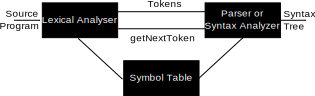
\includegraphics[width=.9\linewidth]{lexical_parser_relation}
		\end{center}
	\vfill
	\item There is three types of parsers for grammars: universal, top-down, bottom-up.
	\item But universal methods, such as the Cocke-Younger-Kasami algorithm and Earley's algorithm, are too inefficient.
	\item The most efficient top-down and bottom-up methods work only for subclasses of grammars: $LL$ and $LR$ grammars.
	\item But $LL$ and $LR$ grammars are expressive enough to describe most of the syntactic constructs in modern programming languages.
	\item $LL$ grammars are commonly used when writing a parser by hands
	\item $LR$ grammars are more complex and used in parser generators.
	\end{itemize}
\end{frame}

\subsection{Error recovery}

\sidecite{Dain.1991}
\begin{frame}{Handling of Syntax Errors}
	\begin{itemize}
	\item A compiler is expected to assist the programmer in locating and tracking down errors that inevitably creep into programs.
	\item Most programming language specifications do not describe how a compiler should respond to errors; error handling is left to the compiler designer.
	\vfill
	\item \alert{Why handling errors during the parsing?} \begin{itemize}
		\item $LL$ and $LR$ methods permits to detect errors efficiently and as soon as possible.
		\item Many errors appear syntactic, whatever they cause, and are exposed when parsing cannot continue.
		\end{itemize}
	\vfill
	\item \alert{The error handler must:} \begin{itemize}
		\item Report the presence of errors clearly and accurately.
		\item Recover from each error quickly to detect subsequent errors.
		\item Add minimal overhead to the processing of correct programs.
		\end{itemize}
	\end{itemize}
\end{frame}

\begin{frame}{Types of Programming Errors}
	\begin{description}
	\item[Lexical errors] they include misspellings of identifiers, keywords, or operators; and missing quotes around text intended as a string.
	\vfill
	\item[Syntactic errors] they include misplaced semicolons or extra or missing braces. Another example is a \kw{case} outside an enclosing \kw{switch} block.
	\vfill
	\item[Semantic errors] they include type mismatches between operators and operands.
	\vfill
	\item[Logical errors] they can be anything from incorrect reasoning on the part of the programmer to the use in a program. For example, the use of the operator \code{"="} in place of the operator \code{"=="}; or unreachable code.
	\end{description}
\end{frame}

\begin{frame}{Strategies for Error Recovery}
	\begin{small}
	\alertbox{Once an error is detected, how should the parser recover?}
	\vfill
	\begin{itemize}
	\item Although no strategy has proven itself universally acceptable.
	\vfill
	\item The simplest approach is for a parser to quit with an informative error message when it detects the first error; additional errors are uncovered.
	\vfill
	\item If errors pile up, it is better for the compiler to give up after exceeding some error limit than to produce an annoying avalanche of ``spurious'' errors.
	\vfill
	\item The rest of this section is devoted to the two major error-recovery strategies: \emph{panic mode}, and \emph{phrase-level recovery}.
	\end{itemize}
	\end{small}
\end{frame}

\begin{frame}{Panic Mode}
	\begin{itemize}
	\item The parser discards input symbols one at a time until one of a designated set of synchronizing tokens is found.
	\vfill
	\item The synchronizing tokens are usually delimiters, such as semicolons or closing braces, whose role in the source program is clear and unambiguous.
	\vfill
	\item This approach is simple to implement and it guarantees not to go into an infinite loop.
	\end{itemize}
\end{frame}

\begin{frame}{Phase-Level Recovery}
	\begin{itemize}
	\item On discovering an error, the parser may perform local correction on the remaining input:
		\begin{itemize}
		\item It may replace the prefix of the remaining input by some string that it allows the parser to continue; eg. replacing a coma by a semicolon, remove extraneous semicolon; or insert a missed semicolon
		\end{itemize}
	\vfill
	\item The choice of the correction is left to the compiler designer.
	\vfill
	\item The major drawback of the phrase-level recovery is the difficulty it has in coping with situations in which the actual error has occurred before the point of detection.
	\end{itemize}
\end{frame}

\begin{frame}{Error Productions}
	\begin{itemize}
	\item To anticipate the error detection, we can augment the grammar for the language at hand with productions that generate the erroneous constructs.
	\vfill
	\item A parser constructed from an augmented grammar detects the anticipated errors when an error production is used during parsing.
	\vfill
	\item The parser can then generate appropriate error diagnostics about the erroneous constructs that has been  recognized in the input.
	\end{itemize}
\end{frame}

\begin{frame}{Global Corrections}
	\begin{itemize}
	\item It would be helpful that a compiler makes few changes as possible in processing an incorrect input string.
	\vfill
	\item Given an incorrect input string \code{x} and grammar $G$, some algorithms find a parse tree for a related string \code{y}, such that the number of insertions, deletions, and changes of tokens required to transform \code{x} to \code{y} is as small as possible.
	\vfill
	\item \emph{Unfortunately, these methods are too costly in time and space.}
	\vfill
	\item Global corrections has been used to evaluate error-recovery algorithms and to find optimal replacement strings for phrase-level recovery.
	\end{itemize}
\end{frame}

\section{Context-free grammar}

\tableofcontentslide[sections={1-4},sectionstyle={show/shaded},subsectionstyle={show/show/hide},subsubsectionstyle={hide/hide/hide/hide}]

\subsection{Definition and notation}

\sidecite{Chomsky.1956, Backus.1959, Naur.1963, Ingerman.1967, Hopcroft.2006}
\begin{frame}[allowframebreaks]{What is a Context-Free Grammar?}
	\alertbox*{Grammars are systematically used to describe the syntax of programming language constructs.}
	\begin{itemize}
	\item A context-free grammar consists of \emph{terminals}, \emph{nonterminals}, a \emph{start symbol}, and \emph{productions}.
	\end{itemize}
	\begin{definition}[Terminal --- Token Name]
		The basic symbols from which strings are formed. \\
		It could be assimilated to a token, replied by the lexical analyzer (see Chapter~\ref{chap:lexical_analysis}).
	\end{definition}
	\begin{definition}[Nonterminals]
		Syntactic variables that denote sets of strings. \\
		The sets of strings denoted by nonterminals help to define the language generated by the grammar. Nonterminals impose a hierarchical structure on the language that is key to syntax analysis and translation.
	\end{definition}
	\begin{definition}[Production]
		The productions of a grammar specify the manner in which the terminals and nonterminals can be combined to form strings. Each production consists of: \begin{enumerate}
		\item A nonterminal called the \emph{head} or left side of the production; this production defines some of the strings denoted by the head.
		\item The symbol "$\rightarrow$" (or "\code{\string:\string:\string=}").
		\item A \emph{body}, or right side, consisting of zero or more terminals and nonterminals. The components of the body describe one way in which strings of the nonterminal at the head can be constructed.
		\end{enumerate}
	\end{definition}
	\begin{definition}[Start Symbol]
		In a grammar, one nonterminal is distinguished as the start symbol, and the set of strings it denotes is the language generated by the grammar. Conventionally, the productions for the start symbol are listed first.
	\end{definition}
\end{frame}

\begin{frame}{General Principles}
	\begin{enumerate}
	\item A grammar derives strings by beginning with the start symbol.
	\item It is repeatedly replacing a nonterminal by the body of a production for that nonterminal.
	\item The terminal strings, that can be derived, form the language defined by the grammar.
	\end{enumerate}
	\vfill
	\alertbox{Parsing is the problem of taking a string of terminals and figuring out how to derive it from the start symbol of the grammar. \\
		If the string cannot be derived, the parser reports a syntax error.}
\end{frame}

\begin{frame}[allowframebreaks]{Conventions on Notation}
	\begin{description}
	\item[These symbols are terminals]\begin{itemize}
		\item Lowercase letters early in the alphabet such as a, b, c, \dots
		\item Operator symbols, such as +, *, \dots
		\item Punctuation symbols, such as parentheses, commas, \dots
		\item The digits 0, \dots, 9.
		\item Boldface strings, such as \tok{id} or \tok{number}.
		\item Underlined strings, such as \underline{id} or \underline{number}.
		\end{itemize}
	\item[These symbols are nonterminals]\begin{itemize}
		\item Uppercase letters, such as A, B, C, \dots
		\item The letter \textit{S} which, when it appears, is usually the start symbol.
		\item Lowercase, italic names such as \textit{expression}, \textit{factor}, \dots
		\end{itemize}
	%
	\framebreak
	%
	\item[Productions] A set of productions $A \bnfbody a_1, A \bnfbody a_2, \dots, A \bnfbody a_k$ with a common head $A$ (call them $A$-productions), may be written $A \bnfbody a_1 \bnfor a_2 \bnfor \dots \bnfor a_k$ the alternatives of $A$.
	\item[Start Symbol] Unless stated otherwise, the head of the first production is the start symbol.
	\item[Others Notations]\begin{itemize}
		\item Uppercase letters late in the alphabet, such as X, Y, Z, represent grammar symbols that is, either nonterminals or terminals.
		\item Lowercase letters late in the alphabet, chiefly u, v, \dots, z, represent (possibly empty) strings of terminals.
		\item Lowercase Greek letters $\alpha$, $\beta$, \dots, represent (possibly empty) strings of grammar symbols.
		\end{itemize}
	\end{description}
\end{frame}

\begin{frame}[fragile]{Example of a Contect-Free Grammar}
	\begin{itemize}
	\item The arithmetic expressions are defined by the following grammar.
	\vfill
	\item The terminals are: \begin{description}
		\item[Operators] \code{+}, \code{-}, \code{*}, \code{/}, \code{(}, \code{)};
		\item[Numbers] \tok{number} stands for any number;
		\item[Identifier] \tok{id} stands for any variable's name.
		\end{description}
	\end{itemize}
	\vfill
	\begin{small}
	\begin{bnf}
	\p{ expression ::= expression \tok+ term}
	\p{            ::= expression \tok- term}
	\p{ term       ::= term \tok* factor}
	\p{            ::= term \tok/ factor}
	\p{            ::= factor}
	\p{ factor     ::= \tok( expression \tok)}
	\p{            ::= \tok{number}}
	\p{            ::= \tok{id}}
	\end{bnf}
	\end{small}
\end{frame}

\subsection{Derivations and Parse Tree}

\tableofcontentslide[sections={1-3},sectionstyle={show/shaded},subsectionstyle={show/shaded/hide},subsubsectionstyle={show/show/hide/hide}]

\subsubsection{Derivations}

\begin{frame}{Derivations}
	\begin{itemize}
	\item From the start symbol, each rewriting step replaces a nonterminal by the body of one of its productions.
	\vfill
	\item Let the example:
		\begin{center}\bnfstyle
			E \bnfbody E \tok+ E \bnfor E \tok* E \bnfor \tok- E \bnfor \tok( E \tok) \bnfor \tok{id}
		\end{center}
	\item The replacement of \textit{E} by \textit{\tok- E} will be described by writing:
		\begin{center}\bnfstyle
			E \deriv \tok- E
		\end{center}
	\item \emph{The symbol \deriv means ``derives in one step''.}
	\begin{example}
		\begin{itemize}
		\item Let a nonterminal \bnftext{A} in the middle of symbols: \bnftext{$\alpha$ A $\beta$}
		\item Let the production: \bnftext{A \bnfbody $\gamma$}
		\item Then: \bnftext{$\alpha$ A $\beta$ \deriv $\alpha$ $\gamma$ $\beta$}
		\end{itemize}
	\end{example}
	\end{itemize}
\end{frame}

\begin{frame}{Sequence of Derivations}
	\begin{definition}
		\begin{itemize}
		\item The sequence of derivations \bnftext{$a_1$ \deriv $a_2$ \deriv \dots \deriv $a_n$} rewrites $a_1$ to $a_n$.
		\item It may also be written: \bnftext{$a_1$ \seqderiv $a_n$}.
		\end{itemize}
	\end{definition}
	\begin{block}{Properties}
		\begin{enumerate}
		\item $\alpha\seqderiv\alpha$, for any string $\alpha$, and
		\item If $\alpha\seqderiv\beta$, and $\beta\deriv\gamma$, then $\alpha\seqderiv\gamma$.
		\end{enumerate}
	\end{block}
\end{frame}

\begin{frame}{Derivation as a Sentence of a Grammar}
	\begin{itemize}
	\item If \bnftext{S \seqderiv a}, where \bnftext{S} is the start symbol of a grammar $G$, we say that \bnftext{a} is a \emph{sentential form of $G$}.
	\vfill
	\item A sentence of $G$ is a sentential form, which is nonterminal.
	\vfill
	\item The language generated by $G$ is its set of sentences.
	\vfill
	\item A string of terminals \bnftext{w} is in $L(G)$ iff \bnftext{S \seqderiv w}. Thus $L(G)$ is said to be a context-free language.
	\end{itemize}
\end{frame}

\begin{frame}{Leftmost and Rightmost Derivations}
	\begin{itemize}
	\item At each step in a derivation, there are two choices to be made:
		\begin{enumerate}
		\item To choose which nonterminal to replace, and
		\item To pick a production with that nonterminal as head.
		\end{enumerate}
	\vfill
	\item To understand how parser work, we shall consider derivations in which the nonterminal to be replaced at each step is chosen as follows: \begin{description}
		\item[Leftmost derivation] the leftmost nonterminal in each sentential form is always chosen. If \bnftext{$\alpha$\deriv$\beta$} is a step in which the leftmost nonterminal in $\alpha$ is replaced, we write \bnftext{$\alpha$\derivlm$\beta$}.
		\item[Rightmost derivation] the rightmost nonterminal is always chosen, we write \bnftext{$\alpha$\derivrm$\beta$}.
		\end{description}
	\end{itemize}
\end{frame}

\begin{frame}[t]{Example of Leftmost Derivations}
	\begin{itemize}
	\item Let the grammar: \\
		\begin{small}
		\begin{bnf}
		\p{E ::= E \tok+ E}
		\p{  ::= E \tok* E}
		\p{  ::= \tok- E}
		\p{  ::= \tok( E \tok)}
		\p{  ::= \tok{id}}
		\end{bnf}
		\end{small}
	\item Let the input string: \texttt{2 + 4 * 6}
	\item Corresponding list of tokens: \tok{id}\tok+\tok{id}\tok*\tok{id}
	\item The leftmost derivations are:
	\end{itemize}
	\putat(160,-131){\mdseries\normalsize\normalcolor
		\begin{tabular}[t]{@{}p{1em}p{1em}l}
		\bnftext{E} & \derivlm & \bnftext{E \tok+ E} \\
		\only<2->{& \derivlm & \bnftext{\tok{id} \tok+ E} \\}
		\only<3->{& \derivlm & \bnftext{\tok{id} \tok+ E \tok* E} \\}
		\only<4->{& \derivlm & \bnftext{\tok{id} \tok+ \tok{id} \tok* E} \\}
		\only<5>{& \derivlm & \bnftext{\tok{id} \tok+ \tok{id} \tok* \tok{id}} \\}
		\end{tabular}
	}
\end{frame}

\begin{frame}[t]{Example of Rightmost Derivations}
	\begin{itemize}
	\item Let the grammar: \\
		\begin{small}
		\begin{bnf}
		\p{E ::= E \tok+ E}
		\p{  ::= E \tok* E}
		\p{  ::= \tok- E}
		\p{  ::= \tok( E \tok)}
		\p{  ::= \tok{id}}
		\end{bnf}
		\end{small}
	\item Let the input string: \texttt{2 + 4 * 6}
	\item Corresponding list of tokens: \tok{id}\tok+\tok{id}\tok*\tok{id}
	\item The leftmost derivations are:
	\end{itemize}
	\putat(160,-131){\mdseries\normalsize\normalcolor
		\begin{tabular}[t]{@{}p{1em}p{1em}l}
		\bnftext{E} & \derivrm & E \bnftext{\tok+ E} \\
		\only<2->{& \derivrm & \bnftext{E \tok+ E \tok* E} \\}
		\only<3->{& \derivrm & \bnftext{E \tok+ E \tok* \tok{id}} \\}
		\only<4->{& \derivrm & \bnftext{E \tok+ \tok{id} \tok* \tok{id}} \\}
		\only<5->{& \derivrm & \bnftext{\tok{id} \tok+ \tok{id} \tok* \tok{id}} \\}
		\end{tabular}
	}
\end{frame}

\subsubsection{Parse Tree}

\tableofcontentslide[sections={1-3},sectionstyle={show/shaded},subsectionstyle={show/shaded/hide},subsubsectionstyle={show/shaded/hide/hide}]

\begin{frame}{What is a Parse Tree?}
	\begin{small}
	\begin{definition}[Parse Tree]
	A parse tree shows how the start symbol of a grammar derives a string. It is a pictorial representation of the productions on an input string of tokens.
	\end{definition}
	\begin{block}{\small Building a Parse Tree}
		\begin{itemize}
		\item The root is labeled by the start symbol.
		\item Each leaf is labeled by a terminal or by $\epsilon$.
		\item Each interior node is labeled by a nonterminal.
		\item If $A$ is the nonterminal of some interior node and $X_1, X_2, \dots, X_n$ are the labels of the children of that node from left to right, then there must be a production $A \bnfbody X_1 X_2 \dots X_n$.
		\end{itemize}
	\end{block}
	\alertbox{Parsing is the process of building a parse tree.}
	\end{small}
\end{frame}

\begin{frame}{Example of a Parse Tree}
	\begin{columns}
		\begin{column}[t]{.5\linewidth}
			Let the string to parse:
				\begin{center}\texttt{9 - 5 + 2}\end{center}
			Let the grammar:\\[1em]
			\begin{scriptsize}
			\begin{bnf}
			\p{ expression ::= expression \tok+ term}
			\p{            ::= expression \tok- term}
			\p{ term       ::= term \tok* factor}
			\p{            ::= term \tok/ factor}
			\p{            ::= factor}
			\p{ factor     ::= \tok( expression \tok)}
			\p{            ::= \tok{number}}
			\p{            ::= \tok{id}}
			\end{bnf}
			\end{scriptsize}
		\end{column}
		\begin{column}[t]{.5\linewidth}
			The parse tree is:\\[1em]
			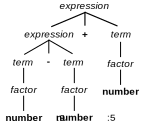
\includegraphics[width=.9\linewidth]{parse_tree_expr}
		\end{column}			
	\end{columns}
\end{frame}

\subsubsection{Building a Parse Tree with Derivations}

\tableofcontentslide[sections={1-3},sectionstyle={show/shaded},subsectionstyle={show/shaded/hide},subsubsectionstyle={show/shaded/hide/hide}]

\begin{frame}[b]{Algorithm to Build a Parse Tree with Derivations}
	\begin{scriptsize}
	\begin{myalgorithm}
	\SetKwFunction{node}{node}
	\SetKwFunction{nodelabel}{label}
	\SetKwFunction{nodechild}{addChild}
	\Input{A sequence of tokens $T$. A grammar $G$ with the start symbol $s_0$.}
	\Output{A parse tree that corresponds to $T$ and $G$.}
	\Begin{
		$r$ \affect \node($s_0$, $T$) ;	$L$ \affect $[r]$ ; $input[r]$ \affect $T$ \;
		\While(\tcc*[f]{Leftmost derivation}){$L = [n].L'$}{
			$L$ \affect $L'$ \;
			\If{$\exists (\nodelabel(n) \bnfbody b) \in G | input[n]$ matches $b$}{
				\ForEach{$\alpha s \beta = b$}{
					$m$ \affect $\omega \in T | (input[\alpha]\;\omega\;input[\beta]) = input[n]$ \;
					$c$ \affect \node($s$) \;
					\nodechild($n$,$c$) \;
					\If{$s$ is nonterminal}{
						$L$ \affect $L.[c]$ \;
						$input[c]$ \affect $m$ \;
					}
				}
			}
		}
		\Return $r$ \;
	}
	\end{myalgorithm}
	\end{scriptsize}
\end{frame}

\begin{frame}[t]{Example of Parse Tree Building}
	\begin{columns}
		\begin{column}[t]{.7\linewidth}
			Let the grammar: \\
			\begin{small}
			\begin{bnf}
			\p{E ::= E \tok+ E}
			\p{  ::= E \tok* E}
			\p{  ::= \tok- E}
			\p{  ::= \tok( E \tok)}
			\p{  ::= \tok{id}}
			\end{bnf}
			\end{small} \\[1em]
			Tokens: {\small \tok{id}\tok+\tok{id}\tok*\tok{id}} \\[1em]
			\begin{small}
			\only<1>{	$L = [E]$}
			\only<2>{	$L = [n].L' = [E]$ \\
					$input =$ \tok{id}\tok+\tok{id}\tok*\tok{id} \\
					$b =$ \bnftext{$E_0$ \tok+ $E_1$} \\
					$input_{E_0} =$ \tok{id} \\
					$input_{E_1} =$ \tok{id}\tok*\tok{id} \\
					$L = [E_0, E_1]$
			}
			\only<3,5>{	$L = [n].L' = [E, E]$ \\
					$input =$ \tok{id} \\
					$b =$ \tok{id} \\
					$L = [E]$
			}
			\only<4>{	$L = [n].L' = [E]$ \\
					$input =$ \tok{id}\tok*\tok{id} \\
					$b =$ \bnftext{$E_0$ \tok* $E_1$} \\
					$input_{E_0} =$ \tok{id} \\
					$input_{E_1} =$ \tok{id} \\
					$L = [E_0, E_1]$
			}
			\only<6>{	$L = [n].L' = [E]$ \\
					$input =$ \tok{id} \\
					$b =$ \tok{id} \\
					$L = []$
			}
			\end{small}
		\end{column}
		\begin{column}[t]{.3\linewidth}
			Parse tree is: \\[1em]
			\includeanimatedfigure[width=\linewidth]{parse_tree_example}
		\end{column}
	\end{columns}
\end{frame}

\subsection{Ambiguity of a grammar}

\tableofcontentslide[sections={1-4},sectionstyle={show/shaded},subsectionstyle={show/shaded/hide},subsubsectionstyle={show/show/hide/hide}]

\sidecite{Cantor.1962, Floyd.1962}
\begin{frame}{What is an Ambiguous Grammar?}
	\begin{small}
	\alertbox*{A grammar that produces more than one parse tree for some sentence is said to be ambiguous.}
	\begin{itemize}
	\item An ambiguous grammar is one that produces more than one leftmost derivation or more than one rightmost derivation for the same sentence.
	\end{itemize}
	\begin{example}
		Leftmost derivations for the arithmetic expression \tok{id}\tok+\tok{id}\tok*\tok{id}.
	\end{example}
	\end{small}
	\begin{tiny}
	\begin{tabular*}{\linewidth}{@{}c@{}|@{}c@{}}
		{\itshape	\begin{tabular}{lcl}
				E & \deriv & E \tok+ E \\
				  & \deriv & \tok{id} \tok+ E \\
				  & \deriv & \tok{id} \tok+ E \tok* E \\
				  & \deriv & \tok{id} \tok+ \tok{id} \tok* E \\
				  & \deriv & \tok{id} \tok+ \tok{id} \tok* \tok{id}
				\end{tabular}
				\raisebox{-.5\height}{\includegraphics[width=.25\linewidth]{ambiguity_2}}
		}
	&
		{\itshape	\begin{tabular}{lcll}
				E & \deriv & E \tok* E \\
				  & \deriv & E \tok+ E \tok* E \\
				  & \deriv & \tok{id} \tok+ E \tok* E \\
				  & \deriv & \tok{id} \tok+ \tok{id} \tok* E \\
				  & \deriv & \tok{id} \tok+ \tok{id} \tok* \tok{id}
				\end{tabular}
				\raisebox{-.5\height}{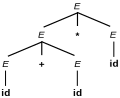
\includegraphics[width=.25\linewidth]{ambiguity_1}}
		}
	\end{tabular*}
	\end{tiny}
\end{frame}

\begin{frame}{Grammar Ambiguity is not Desirable}
	\begin{itemize}
	\item For parsers, it is desirable that the grammar be made unambiguous. Otherwise we cannot determine which parse tree to select for a sentence.
	\vfill
	\item Another way is to use carefully chosen ambiguous grammars, together with \emph{disambiguating rules} that discard undesirable parse trees, leaving only one tree for each sentence.
	\end{itemize}
\end{frame}

\subsection{Verifying the language supported by a grammar}

\tableofcontentslide[sections={1-4},sectionstyle={show/shaded},subsectionstyle={show/shaded/hide},subsubsectionstyle={show/show/hide/hide}]

\begin{frame}{Verifying the Language Supported by a Grammar}
	\begin{small}
	\begin{itemize}
	\item Even if compiler designers rarely do this task, it is useful to be able to verify if a language can be generated from a grammar.
	\vfill
	\item A proof that a grammar $G$ generates a language $L$ has two parts:
		\begin{enumerate}
		\item Show that every string generated by $G$ is in $L$.
		\item Show that every string in $L$ can be generated by $G$.
		\end{enumerate}
	\end{itemize}
	\begin{example}
		Considerer the following grammar:
		\begin{center}\bnfstyle S \bnfbody \tok( S \tok) S \bnfor \tok{e}\end{center}
		It may not be apparent, but this grammar generates all the strings of balanced parentheses, and only such strings.  That why, we need to proceed the two steps of the proof.
	\end{example}
	\end{small}
\end{frame}

\begin{frame}{Part 1: every string generated by $G$ is in $L$}
	\begin{description}
	\item[BASIS] The basis is $n=1$. The only string of terminals derivable from $S$ in one step is the empty string, which is balanced.
	\item[INDUCTION] Assume that all derivations of fewer than $n$ steps produce balanced sentences, and consider a leftmost derivation of exactly $n$ steps. Such a derivation must be of the form:
		\begin{center}\bnfstyle S \derivlm \tok( S \tok) S \derivlm \tok( x \tok) S \derivlm \tok( x \tok) y\end{center}
		The derivations of x and y from $S$ take fewer than $n$ steps, so by the inductive hypothesis $x$ and $y$ are balanced. Therefore, the string $\tok(x\tok)y$ must be balanced.
	\end{description}
\end{frame}

\begin{frame}{Part 2: every string in $L$ can be generated by $G$}
	\begin{description}
	\item[BASIS] If the string is length $0$, it must be $\epsilon$, which is balanced.
	\item[INDUCTION] Observe that every balanced string has even length. Assume that every balanced string of length less than $2n$ is derivable from $S$, and consider a balanced string $w$ of length $2n$, $n\ge1$. Surely $w$ begins with a left parenthesis. \\
		Let \bnftext{\tok(x\tok)} be the shortest nonempty prefix of $w$ having an equal number of left and right parentheses. \\
		Then $w$ can be written \bnftext{w = \tok(x\tok)y} where both $x$ and $y$ are balanced. Since $x$ and $y$ are of length less than $2n$, they are derivable from $S$ by the inductive hypothesis. Thus, we can find a derivation of the form:
			\begin{center}\bnfstyle S \deriv \tok( S \tok) S \seqderiv \tok( x \tok) S \seqderiv \tok( x \tok) y\end{center}
		proving that \bnftext{w = \tok(x\tok)y} is also derivable from $S$.
	\end{description}
\end{frame}

\subsection{Context-free grammar and regular expression}

\tableofcontentslide[sections={1-4},sectionstyle={show/shaded},subsectionstyle={show/shaded/hide},subsubsectionstyle={show/show/hide/hide}]

\begin{frame}{Context-Free Grammar \vs Regular Expression}
	\begin{itemize}
	\item \emph{Grammars are more powerful notation than regular expressions.}
	\item Every construct that can be described by a regular expression can be described by a grammar, but not vice-versa.
	\item For example the regular expression $(a|b)*abb$ and the following grammar describe the same language. \\
		\begin{bnf}
		\p{$A_0$ ::= \tok{a} $A_0$ \bnfor \tok{b} $A_0$ \bnfor \tok{a} $A_1$}
		\p{$A_1$ ::= \tok{b} $A_2$}
		\p{$A_2$ ::= \tok{b} $A_3$}
		\p{$A_3$ ::= $\epsilon$}
		\end{bnf}
	\item In the other hand, the language $L = { a^nb^n | n \ge 1 }$ is an example of a language that can be described by a grammar but not by a regular expression (except for Posix extension).
	\end{itemize}
\end{frame}

\begin{frame}{From Nondeterministic Finite Automaton to Grammar}
	\begin{itemize}
	\item It is possible to construct a grammar from a regular expression through the corresponding NFA.
	\vfill
	\item This mechanical transformation follows the steps below: \begin{enumerate}
		\item For each state $i$ of the NFA, create a nonterminal $A_i$.
		\item If state $i$ has a transition to state $j$ on input $a$, add the production \bnftext{$A_i$ \bnfbody a$A_j$}. If state $i$ goes to state $j$ on input $\epsilon$, add the production \bnftext{$A_i$ \bnfbody $A_j$}.
		\item If $i$ is an accepting state, add \bnftext{$A_i$ \bnfbody $\epsilon$}.
		\item If $i$ is the state state, make $A_i$ be the start symbol of the grammar.
		\end{enumerate}
	\end{itemize}
\end{frame}

\subsection{Guidelines for writing a grammar}

\subsubsection{General guidelines}

\tableofcontentslide[sectionstyle={show/shaded},subsectionstyle={show/shaded/hide},subsubsectionstyle={show/show/hide/hide}]

\begin{frame}[allowframebreaks]{General Guidelines for Writing a Grammar}
	\begin{itemize}
	\item Grammars are capable of describing most, but not all, of the syntax of programming languages.
		\begin{itemize}
		\item The requirement that identifiers be declared before they are used cannot be described in a grammar.
		\end{itemize}
	\item As seen previously, everything that can be described with a regular expression, can also be described y a grammar.
	\item Why use regular expressions to define the lexical syntax of a language?
		\begin{enumerate}
		\item Separating the syntactic structure of a language into lexical and non-lexical parts provides a better modularity.
		\item The lexical rules of a language are frequently quite simple, and to describe them we do not need a notation as complex as the grammars.
		\item Regular expressions generally provide a more concise and easier-to-understand notation for tokens than grammars.
		\item More efficient lexical analyzers can be constructed automatically from regular expressions than from arbitrary grammars.
		\end{enumerate}
	\item There a no firm guidelines as to what to put into the lexical rules, as opposed to the syntactic rules.
	\item Regular expressions are useful to describe constructs such as identifiers, numbers\dots
	\item Grammars are most useful for describing nested structures such as balanced parentheses, corresponding if-then-else\dots
	\end{itemize}
\end{frame}

\subsubsection{Eliminating the ambiguity}

\tableofcontentslide[sectionstyle={show/shaded},subsectionstyle={show/shaded/hide},subsubsectionstyle={show/shaded/hide/hide}]

\begin{frame}[t,allowframebreaks]{Example of Ambiguity Elimination: ``dangling else''}
	\begin{footnotesize}
	\alertbox{An ambiguous grammar can be rewritten to eliminate the ambiguity.}
	\begin{description}
	\item[Grammar]
			\begin{bnf}
			\p{statement ::= \tok{if} expression \tok{then} statement}
			\p{          ::= \tok{if} expression \tok{then} statement \tok{else} statement}
			\p{          ::= \tok{other}}
			\end{bnf}
	\item[Input] \tok{if} $E_1$ \tok{then} \tok{if} $E_2$ \tok{else} $S_1$ \tok{else} $S_2$
	\end{description}
	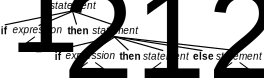
\includegraphics[width=.55\linewidth]{ambiguity_3}\hfill
	\includegraphics[width=.45\linewidth]{ambiguity_4}
	\begin{itemize}
	\item The first tree is preferred according to ``Match each \tok{else} with the closest unmatched \tok{then}.'' This rule is rarely built into productions.
	\end{itemize}
	\end{footnotesize}
	%
	\framebreak
	%
	\begin{footnotesize}
	The disambiguation of this ``if-then-else'' problem may be included into a new grammar.
	\begin{bnf}
	\p{statement ::= \tok{if} expression \tok{then} statement}
	\p{          ::= \tok{if} expression \tok{then} statement \tok{else} statement}
	\p{          ::= \tok{other}}
	\end{bnf}
	\begin{center}
\includegraphics[height=3em]{bottomarrow}\end{center}
	\begin{bnf}
	\p{statement ::= matched\_statement}%\tok{if} expression \tok{then} statement}
	\p{          ::= open\_statement}%
	\p{matched\_statement ::= \tok{if} expression \tok{then} matched\_statement \tok{else} matched\_statement}
	\p{                   ::= \tok{other}}
	\p{open\_statement ::= \tok{if} expression \tok{then} statement}
	\p{                ::= \tok{if} expression \tok{then} matched\_statement \tok{else} open\_statement}
	\end{bnf}
	\end{footnotesize}
\end{frame}

\subsubsection{Eliminating the left recursion}

\tableofcontentslide[sectionstyle={show/shaded},subsectionstyle={show/shaded/hide},subsubsectionstyle={show/shaded/hide/hide}]

\begin{frame}{Left Recursive Grammar}
	\begin{definition}[Left-Recursive Grammar]
		A grammar is left recursive if it has a nonterminal A such that there is a derivation $A \seqderivone A\alpha$ for some string $\alpha$.
	\end{definition}
	\alertbox{Top-down parsing methods cannot handler left-recursive grammars.}
	\begin{itemize}
	\vfill
	\item \emph{A transformation is needed to eliminate left recursion.}
	\vfill
	\item The algorithm to systematically eliminates left recursion from a grammar if the grammar has no cycle nor $\epsilon$-production: \begin{itemize}
		\item $\neg\left(A \seqderivone A\right)$ --- no cycle
		\item $\neg\left(A \bnfbody \epsilon\right)$ --- no $\epsilon$-production
		\end{itemize}
	\end{itemize}
\end{frame}

\begin{frame}{Eliminating Left Recursion}
	\begin{small}
	\begin{myalgorithm}
	\Input{Grammar $G$.}
	\Output{An equivalent grammar with no left recursion.}
	\Begin{
		\While{$\exists A | (A \bnfbody A\;\gamma) \in G$}{
			\ForEach{$p = (A \bnfbody b\;\delta) \in G | b \neq A$}{
				$G \affect G \setminus \{ p \}$ \;
				$G \affect G \cup \left\{ (R_A \bnfbody b\;\delta\;R_A) \right\}$ \;
			}
			$G = G \cup \left\{ (R_A \bnfbody \epsilon) \right\}$ \;
			\ForEach{$p = (A \bnfbody A\;\omega) \in G$}{
				$G \affect G \setminus \{ p \}$ \;
				$G \affect G \cup \left\{ (A \bnfbody \omega\;R_A) \right\}$ \;
			}
		}
	}
	\end{myalgorithm}
	\end{small}
\end{frame}

\begin{frame}{Example of Eliminating Left Recursion}
	\begin{tabularx}{\linewidth}{@{}XcX@{}}
		\begin{bnf}
		\p{E ::= E \tok+ E}
		\p{  ::= E \tok* E}
		\p{  ::= \tok- E}
		\p{  ::= \tok( E \tok)}
		\p{  ::= \tok{id}}
		\end{bnf}
	&
		\includegraphics[width=3em]{rightarrow}
	&
		\begin{bnf}
		\p{E ::= \tok- E $R_E$}
		\p{  ::= \tok( E \tok) $R_E$}
		\p{  ::= \tok{id} $R_E$}
		\p{$R_E$ ::= \tok+ E $R_E$}
		\p{      ::= \tok* E $R_E$}
		\p{      ::= \ensuremath{\epsilon}}
		\end{bnf}
	\end{tabularx}
\end{frame}

\subsubsection{Left factoring}

\tableofcontentslide[sectionstyle={show/shaded},subsectionstyle={show/shaded/hide},subsubsectionstyle={show/shaded/hide/hide}]

\begin{frame}{Left Factoring}
	\begin{itemize}
	\item When the choice between two alternatives $A$-productions is not clear, we may be able to rewrite the productions to defer the decision until enough of the input has been seen that we can make the right choice.
	\end{itemize}
	\vfill
	\begin{small}\begin{center}
		\begin{bnf}[.9\linewidth]
		\p{statement ::= \tok{if} expression \tok{then} statement \tok{else} statement}
		\p{          ::= \tok{if} expression \tok{then} statement}
		\p{          ::= \tok{other}}
		\end{bnf}
	\end{center}\end{small}
	\vfill
	\alertbox*{Left factoring is a grammar transformation that is useful for producing a grammar suitable for predictive, or top-down, parsing.}
\end{frame}

\begin{frame}{Example of Left Factoring}
	\begin{small}\begin{center}
		\begin{bnf}[.9\linewidth]
		\p{statement ::= \tok{if} expression \tok{then} statement \tok{else} statement}
		\p{          ::= \tok{if} expression \tok{then} statement}
		\p{          ::= \tok{other}}
		\end{bnf} \\[1em]
		
\includegraphics[height=3em]{bottomarrow} \\[1em]
		\begin{bnf}[.95\linewidth]
		\p{statement ::= \tok{if} expression \tok{then} statement else\_statement}
		\p{          ::= \tok{other}}
		\p{else\_statement ::= \tok{else} statement}
		\p{                  ::= $\epsilon$}
		\end{bnf}
	\end{center}\end{small}
\end{frame}

\begin{frame}{Algorithm for Left Factoring}
	\begin{small}
	\begin{myalgorithm}
	\Input{Grammar $G$.}
	\Output{An equivalent left-factored grammar.}
	\BlankLine
	\Begin{
		\While{$\exists A  \in G | (A \bnfbody \alpha\;\gamma), (A \bnfbody \alpha\;\delta)$}{
			\ForEach{$p = (A \bnfbody \alpha\;\omega) \in G$}{
				$G \affect G \setminus \{ p \}$ \;
				\If{$\omega \neq \epsilon$}{
					$G \affect G \cup \left\{ (R_A \bnfbody \omega) \right\}$ \;
				}
			}
			$G \affect G \cup \left\{ (A \bnfbody \alpha\;R_A) \right\}$ \;
			$G \affect G \cup \left\{ (R_A \bnfbody \epsilon) \right\}$ \;
		}
	}
	\end{myalgorithm}
	\end{small}
\end{frame}

\section{Parsing with a grammar}

\tableofcontentslide[sectionstyle={show/shaded},subsectionstyle={show/show/hide},subsubsectionstyle={hide/hide/hide/hide}]

\subsection{Top-down parsing}

\tableofcontentslide[sectionstyle={show/shaded},subsectionstyle={show/shaded/hide},subsubsectionstyle={show/show/hide/hide}]

\subsubsection{Principles}

\begin{frame}{Top-Down Parsing}
	\begin{itemize}
	\item Top-down parsing can be viewed as the problem of constructing a parse tree for the input string, starting from the root and creating the nodes of the parse tree in preorder.
	\item Top-down parsing can be viewed as finding a leftmost derivation for an input string.
	\item The rest of this section uses the following grammar as illustration; and uses the input string \tok{id}\tok+\tok{id}\tok*\tok{id}.
	\end{itemize}
	\begin{small}
	\begin{center}
		\begin{bnf}[.4\linewidth]
		\p{E  ::= T E'}
		\p{E' ::= \tok+ T E'}
		\p{   ::= $\epsilon$}
		\p{T  ::= F T'}
		\p{T' ::= \tok* F T'}
		\p{   ::= $\epsilon$}
		\p{F  ::= \tok( E \tok)}
		\p{   ::= \tok{id}}
		\end{bnf}
	\end{center}
	\end{small}
\end{frame}

\begin{frame}{Types of Top-Down Parsing}
	\begin{itemize}
	\item Several top-down parsing methods exist, the two majors are:
		\begin{description}
		\vfill
		\item[Recursive-descent parsing] a general form, which may require backtracking to find the correct $A$-production to be applied.
		\vfill
		\item[Predictive parsing] a special case of recursive-descent parsing, where no backtracking is required. The $A$-production is chosen by looking ahead at the input a fixed number of symbols.
		\end{description}
	\vfill
	\item The class of grammars dedicated to the predictive parsers looking $k$ symbols ahead in the input is called $LL(k)$ class.
	\end{itemize}
\end{frame}

\subsubsection{Recursive-descent parsing}

\tableofcontentslide[sectionstyle={show/shaded},subsectionstyle={show/shaded/hide},subsubsectionstyle={show/shaded/hide/hide}]

\sidecite{Hoare.1962, Schorre.1964, McClure.1965}
\begin{frame}{Recursive-Descent Parsing}
	\begin{itemize}
	\item A recursive-descent parsing program consists of a set of procedures, one for each nonterminal.
	\vfill
	\item Execution begins with the procedure for the start symbol.
	\vfill
	\item The pseudo-code for each nonterminal is:
		\begin{scriptsize}
		\begin{myprocedure}{$A$}{}
		\SetKwFunction{call}{call}
		\Input{A production $A \bnfbody \alpha_1\dots\alpha_k$.}
		\Begin{
			\For{$i$ \affect $1$ \KwTo $k$}{
				\uIf{$\alpha_i$ is a nonterminal}{
					\call $\alpha_i$() \;
				}
				\uElseIf{$\alpha_i = $current input symbol $a$}{
					forward \affect forward + 1 \tcp*[f]{Move input pointer}\;
				}
				\Else{
					Report an error \;
				}
			}
		}
		\end{myprocedure}
		\end{scriptsize}
	\end{itemize}
\end{frame}

\begin{frame}{Problem of Infinite Loop}
	\begin{itemize}
	\item A left-recursive grammar can cause a recursive-descent parser to go into an infinite loop.
	\item That is, when we try to expand a nonterminal $A$, we may eventually find ourselves again trying to expand $A$ without having consumed input.
	\end{itemize}
	\vfill
	\begin{columns}
		\begin{column}{.5\linewidth}
			\begin{bnf}
			\p{E ::= E \tok+ E}
			\p{  ::= E \tok* E}
			\p{  ::= \tok- E}
			\p{  ::= \tok( E \tok)}
			\p{  ::= \tok{id}}
			\end{bnf}
		\end{column}
		\begin{column}{.5\linewidth}\bnfstyle
			\begin{tabular}{@{}ll@{}}
				E & \deriv E \tok+ E \\
				E & \deriv E \tok+ E \tok+ E \\
				E & \deriv E \tok+ E \tok+ E \tok+ E \\
				E & \deriv E \tok+ E \tok+ E \tok+ E \tok+ E \\
				& \deriv \dots
			\end{tabular}
		\end{column}
	\end{columns}	
\end{frame}

\subsubsection{FIRST and FOLLOW}

\tableofcontentslide[sectionstyle={show/shaded},subsectionstyle={show/shaded/hide},subsubsectionstyle={show/shaded/hide/hide}]

\begin{frame}{What are the Functions FIRST and FOLLOW?}
	\begin{itemize}
	\item The construction of both top-down and bottom-up parsers is aided by two functions associated with a grammar G:
		\begin{enumerate}
		\item FIRST
		\item FOLLOW
		\end{enumerate}
	\vfill
	\item These functions allow us to choose which production to apply, based on the next input symbol.
	\vfill
	\item During panic-mode error recovery the set of tokens replied by FOLLOW can be used as synchronizing tokens.
	\end{itemize}
\end{frame}

\begin{frame}{Definition of FIRST}
	\begin{itemize}
	\item Define FIRST($\alpha$), where $\alpha$ is any string of grammar symbols, to be the set of terminals that begin strings derived from $\alpha$.
	\item If $\alpha \seqderiv \epsilon$, then $\epsilon$ is also in FIRST($\alpha$).
	\end{itemize}
	\vfill
	\begin{example}\bnfstyle
		\begin{columns}
			\begin{column}[t]{.4\linewidth}
				$A \seqderiv c\;\gamma$ \\
				FIRST($A$) $ = \{ c \}$
			\end{column}
			\begin{column}[t]{.4\linewidth}
				\raisebox{-\height}{\includegraphicswtex[width=\linewidth]{example_FIRST}}
			\end{column}
		\end{columns}
	\end{example}
\end{frame}

\begin{frame}{Algorithm of FIRST}
	\begin{itemize}
	\item To compute FIRST($X$) for a grammar symbol $X$, apply the following rules until no more terminals or $\epsilon$ can be added to any FIRST set.
	\vfill
		\begin{enumerate}
		\item If $X$ is a terminal, then FIRST($X$) $= \{ X \}$.
		\item If $X$ is a nonterminal and $X \bnfbody Y_1\;Y_2 \dots Y_k$ is a production for some $k \ge 1$, then place $a$ in FIRST($X$) if for some $i$, $a$ is in FIRST($Y_i$), and $\epsilon$ is in all of FIRST($Y_1$), \dots, FIRST($Y_{k-1}$); that is, $Y_1\;Y_2 \dots Y_k \seqderiv \epsilon$. If $\epsilon$ is in FIRST($Y_j$) for all $j \in \{1, 2, \dots, k\}$, then add $\epsilon$ to FIRST($X$).
		\item If $X \bnfbody \epsilon$ is a production, then add $\epsilon$ to FIRST($X$).
		\end{enumerate}
	\vfill
	\item Add to FIRST($X_1\;X_2 \dots X_n$) all non-$\epsilon$ symbols of FIRST($X_i$) for $i \in \{1 \dots n\}$.
	\end{itemize}
\end{frame}

\begin{frame}{Definition of FOLLOW}
	\begin{scriptsize}
	\begin{itemize}
	\item Define FOLLOW($A$), where $A$ is a nonterminal, to be the set of terminals a that can appear immediately to the right of $A$ in some sentential form.
	\item The set of terminals a such that there exists a derivation of the form $S \seqderiv \alpha\;A\;a\;\beta$, for some $\alpha$ and $\beta$.
	\item Note that there may have been symbols between $A$ and $a$, at some time during the derivation, but if so, they derive $\epsilon$ and disappeared.
	\item If $A$ can be the rightmost symbol, then \tok{eof} (or usually \tok{\$}) is in FOLLOW($A$).
	\end{itemize}
	\end{scriptsize}
	\vfill
	\begin{small}
	\begin{example}\bnfstyle
		\begin{columns}
			\begin{column}[t]{.4\linewidth}
				$A \seqderiv c\;\gamma$ \\
				$a \in $FOLLOW($A$)
			\end{column}
			\begin{column}[t]{.4\linewidth}
				\raisebox{-\height}{\includegraphicswtex[width=\linewidth]{example_FIRST}}
			\end{column}
		\end{columns}
	\end{example}
	\end{small}
\end{frame}

\begin{frame}{Algorithm of FOLLOW}
	\begin{itemize}
	\item To compute FOLLOW($A$) for a nonterminal $A$, apply the following rules until nothing can be added to any FOLLOW set.
		\begin{enumerate}
		\vfill
		\item Place \tok{eof} in FOLLOW($S$), where $S$ is the start symbol, and \tok{eof} is the input right endmarker.
		\vfill
		\item If there is a production \bnftext{A \bnfbody $\alpha\;B\;\beta$}, then everything in FIRST($b$), except $\epsilon$ is in FOLLOW($B$).
		\vfill
		\item If there is a production \bnftext{A \bnfbody $\alpha\;B$}, or a production \bnftext{A \bnfbody $\alpha\;B\;\beta$}, where FIRST($\beta$) contains $\epsilon$, then everything in FOLLOW($A$) is in FOLLOW($B$).
		\end{enumerate}
	\end{itemize}
\end{frame}

\subsubsection{$LL(1)$ grammars}

\tableofcontentslide[sectionstyle={show/shaded},subsectionstyle={show/shaded/hide},subsubsectionstyle={show/shaded/hide/hide}]

\sidecite{Lewis.1968, Birman.1973}
\begin{frame}{$LL(1)$ Grammar}
	\begin{itemize}
	\item Predictive parsers, that is, recursive-descent parsers needing no backtracking, can be constructed for a class of grammars called $LL(1)$.
	\vfill
		\begin{itemize}
		\item \Emph{L}eft-to-right input scanning,
		\item \Emph{L}eftmost derivation,
		\item \Emph{1} input symbol is used for lookahead to make parsing action decisions.
		\end{itemize}
	\vfill
	\item The class of $LL(1)$ grammars is rich enough to cover most programming constructs, although care is needed in writing a suitable grammar for the source language \eg no left-recursive nor ambiguous grammar can be $LL(1)$.
	\end{itemize}
\end{frame}

\begin{frame}{Definition of a $LL(1)$ Grammar}
	\begin{itemize}
	\item A grammar $G$ is $LL(1)$ iff whenever \bnftext{A \bnfbody $\alpha$ \bnfor $\beta$} are two distinct productions of $G$, the following conditions hold:
		\begin{enumerate}
		\vfill
		\item For nonterminal $a$ do both $\alpha$ and $\beta$ derive strings beginning with $a$.
		\vfill
		\item At most one of $\alpha$ and $\beta$ can derive the empty string.
		\vfill
		\item If $\beta\seqderiv\epsilon$, then $\alpha$ does not derive any string beginning with a terminal in FOLLOW($A$). Likewise, if $\alpha\seqderiv\epsilon$, then $\beta$ does not derive any string beginning with a terminal in FOLLOW($A$).
		\end{enumerate}
	\end{itemize}
	\vfill
	\begin{small}
	\begin{bnf}
	\p{statement\_list ::= statement statement\_list}
	\p{                ::= $\epsilon$}
	\p{statement ::= \tok{if} \tok( expression \tok) statement \tok{else} statement}
	\p{          ::= \tok{while} \tok( expression \tok) statement}
	\p{          ::= \tok\{ statement\_list \tok\}}
	\end{bnf}
	\end{small}
\end{frame}

\begin{frame}{Parsing a $LL(1)$ Grammar}
	\alertbox{To parse an input string, a table should be build. It permits to determine the production to use from a given production and the input symbol.}
	\vfill
	\begin{itemize}
	\item The following algorithm permits to collects informations from FIRST and FOLLOW sets into a predictive parsing table $M[A,a]$, where $A$ is a nonterminal, and $a$ is a terminal or \tok{eof}.
	\end{itemize}
\end{frame}

\begin{frame}[allowframebreaks]{Algorithm for Building the Predicitve-Parsing Table}
	\vfill
	\begin{itemize}
	\item The algorithm is based on the idea:
		\begin{enumerate}
		\item The production \bnftext{A \bnfbody $\alpha$} is chosen if the next input symbol $a \in $FIRST($\alpha$).
		\item When $\alpha\seqderiv\epsilon$, we should again choose \bnftext{A \bnfbody $\alpha$}, of the current input symbol is in FOLLOW($A$), or if the \tok{eof} on the input has been reached and \tok{eof} is in FOLLOW($A$).
		\end{enumerate}
	\vfill
	\item If a cell of the predictive parsing table contains more than one information, then the grammar associated to the table is ambiguous.
	\end{itemize}
	\vfill
	%	
	\framebreak
	%
	\begin{description}
	\item[INPUT] Grammar $G$.
	\item[OUTPUT] Parsing table $M$.
	\item[METHOD] For each production \bnftext{A \bnfbody $\alpha$} of the grammar, do the following:
		\begin{itemize}
		\item For each terminal $a$ in FIRST($\alpha$), add \bnftext{A \bnfbody $\alpha$} to $M[A,a]$.
		\item If $\epsilon$ is in FIRST($\alpha$), then for each terminal $b$ in FOLLOW($A$), add \bnftext{A \bnfbody $\alpha$} to $M[A,b]$.
		\item If $\epsilon$ is in FIRST($\alpha$) and \tok{eof} is in FOLLOW($A$), add \bnftext{A \bnfbody $\alpha$} to $M[A,\tok{eof}]$ as well.
		\end{itemize}
		\vspace{1em}
		If, after performing the above, there is no production in $M[A,a]$, then set $M[A,a]$ to error (generally replaced by an empty string in the table).
	\end{description}
\end{frame}

\begin{frame}[t]{Example of Table Building}
	\begin{scriptsize}
	\begin{bnf}[.33\linewidth]
	\p[1]{E  ::= T E'}
	\p[2]{E' ::= \tok+ T E'}
	\p[3]{   ::= $\epsilon$}
	\p[4]{T  ::= F T'}
	\p[5]{T' ::= \tok* F T'}
	\p[6]{   ::= $\epsilon$}
	\p[7]{F  ::= \tok( E \tok)}
	\p[8]{   ::= \tok{id}}
	\end{bnf}
	\end{scriptsize} \\[1em]
	\begin{small}\bnfstyle
	\begin{tabularx}{\linewidth}{|c|X|X|X|X|X|X|}
		\hline
		\tabularheading&\chead{\tok{id}}&\chead{\tok+}&\chead{\tok*}&\chead{\tok(}&\chead{\tok)}&\chead{\tok{eof}} \\
		\hline
		E & \only<2->{\bnfmark{1}} & & & \only<2->{\bnfmark{1}} & & \\
		\hline
		E' & & \only<3->{\bnfmark{2}} & & & \only<4->{\bnfmark{3}} & \only<5->{\bnfmark{3}} \\
		\hline
		T & \only<6->{\bnfmark{4}} & & & \only<6->{\bnfmark{4}} & & \\
		\hline
		T' & & \only<8->{\bnfmark{6}} & \only<7->{\bnfmark{5}} & & \only<8->{\bnfmark{6}} & \only<8->{\bnfmark{6}} \\
		\hline
		F & \only<10->{\bnfmark{8}} & & & \only<9->{\bnfmark{7}} & & \\
		\hline
	\end{tabularx}
	\end{small}
	\begin{scriptsize}
	\putat(110,-10){\parbox[t]{.55\paperwidth}{\normalfont\normalcolor\small
		\only<1-2>{	\Emph{For production:} \bnfmark{1}~\bnftext{E \bnfbody T E'} \\
				FIRST($T E'$) = FIRST($T$) = FIRST($F$) = $\{ \tok(, \tok{id} \}$ \\
				\only<2>{Then put the production in $M[E,\tok(]$ and $M[E,\tok{id}]$; the rest of the line is \emph{error}}
		}
		\only<3>{	\Emph{For production:} \bnfmark{2}~\bnftext{E' \bnfbody \tok+ T E'} \\
				FIRST($\tok+ T E'$) = $\{ \tok+ \}$ \\
				Then put the production in $M[E',\tok+]$
		}
		\only<4,5>{	\Emph{For production:} \bnfmark{3}~\bnftext{E' \bnfbody $\epsilon$} \\
				FIRST($\epsilon$) = $\{ \epsilon \}$ \\
				FOLLOW($E'$) = $\{ \tok), \tok{eof} \}$ \\
				Put the production in $M[E',\tok)]$ (rule 2) \\
				\only<5>{Put the production in $M[E',\tok{eof}]$ (rule 3)}
		}
		\only<6>{	\Emph{For production:} \bnfmark{4}~\bnftext{T \bnfbody F T'} \\
				FIRST($F\;T'$) = FIRST($F$) = $\{ \tok(, \tok{id} \}$ \\
				Put the production in $M[T,\tok(]$ and $M[T,\tok{id}]$
		}
		\only<7>{	\Emph{For production:} \bnfmark{5}~\bnftext{T' \bnfbody \tok* F T'} \\
				FIRST($\tok*\;F\;T'$) = $\{ \tok* \}$ \\
				Put the production in $M[T',\tok*]$
		}
		\only<8>{	\Emph{For production:} \bnfmark{6}~\bnftext{T' \bnfbody $\epsilon$} \\
				FIRST($\epsilon$) = $\{ \epsilon \}$ \\
				FOLLOW($T'$) = $\{ \tok+, \tok), \tok{eof} \}$ \\
				Put the production in $M[T',\tok+]$ and $M[T,\tok)]$ (rule 2) \\
				Put the production in $M[T',\tok{eof}]$ (rule 3)
		}
		\only<9>{	\Emph{For production:} \bnfmark{7}~\bnftext{F \bnfbody \tok( E \tok)} \\
				FIRST($\tok(\;E\tok)$) = $\{ \tok( \}$ \\
				Put the production in $M[F,\tok(]$
		}
		\only<10>{	\Emph{For production:} \bnfmark{9}~\bnftext{F \bnfbody \tok{id}} \\
				FIRST(\tok{id}) = $\{ \tok{id} \}$ \\
				Put the production in $M[F,\tok{id}]$
		}
	}}
	\end{scriptsize}
\end{frame}

\subsubsection{Nonrecursive predictive parsing}

\tableofcontentslide[sectionstyle={show/shaded},subsectionstyle={show/shaded/hide},subsubsectionstyle={show/shaded/hide/hide}]

\begin{frame}{Nonrecursive Predictive Parsing}
	\begin{itemize}
	\item A nonrecursive predictive parser can be built by maintaining a stack explicitly, rather than implicitly via recursive calls.
	\item The parser mimics a leftmost derivation. If \code{w} is the input that has been matched so far, then the stack holds a sequence of grammar symbols a such that:
		\begin{center}
			$S \seqderiv w\;\alpha$
		\end{center}
	\item The table-driven parser has an \emph{input buffer}, a \emph{stack} containing a sequence of grammar symbols, a \emph{parsing table}, and an \emph{output stream}.
	\end{itemize}
	\begin{center}
		\includegraphics[width=.8\linewidth]{nonrecursive_predictive_parser}
	\end{center}
\end{frame}

\begin{frame}{Algorithm of the Nonrecursive Predictive Parsing}
	\begin{tiny}
	\begin{myalgorithm}
	\SetKwFunction{inputSymbol}{inputSymbol}
	\SetKwFunction{nextInputSymbol}{nextInputSymbol}
	\SetKwFunction{pop}{pop}
	\SetKwFunction{push}{push}
	\SetKwFunction{topOf}{topOf}
	\SetKwFunction{print}{print}
	\Input{A string \code{w}, a parsing table $M$ for grammar $G$, and a start symbol $s_0$.}
	\Output{If \code{w} is in $L(G)$, a lefmost derivation of \code{w}; otherwise, an error indication.}
	\Begin{
		$a$ \affect \inputSymbol()\;
		\push($S$, \tok{eof}) \;
		\push($S$, $s_0$) \;
		\While{$\topOf(S) \neq \tok{eof}$}{
			$X$ \affect \topOf($S$) \;
			\uIf{$X = a$}{
				\pop($S$); $a$ \affect \nextInputSymbol()\;
			}
			\uElseIf{$X$ is a terminal}{
				Report an error\;
			}
			\uElseIf{$M[X,a] = X \bnfbody Y_1 \dots Y_n$}{
				\print($X \bnfbody Y_1 \dots Y_n$)\;
				\pop($S$)\;
				\lFor{$i$ \affect $n$ \KwTo $1$}{\push($S, Y_i$)} \;
			}
			\Else{
				 Report an error\tcp*[f]{$M[X,a]$ is empty}\;
			}
		}
	}
	\end{myalgorithm}
	\end{tiny}
\end{frame}

\pgfdeclareimage[width=2em]{rightarrow_2em}{imgs/all/rightarrow}

\begin{frame}{Example of Nonrecursive Predictive Parsing}
	\only<1>{\putat(-30,-27){\pgfuseimage{rightarrow_2em}}}
	\only<2>{\putat(-30,-34){\pgfuseimage{rightarrow_2em}}}
	\only<3>{\putat(-30,-41){\pgfuseimage{rightarrow_2em}}}
	\only<4,8,12,16,18,22>{\putat(-30,-53){\pgfuseimage{rightarrow_2em}}}
	\only<5,9,13,19,23>{\putat(-30,-94){\pgfuseimage{rightarrow_2em}}}
	\only<6,10,14,20,24>{\putat(-30,-101){\pgfuseimage{rightarrow_2em}}}
	\only<7,11,15,21,25>{\putat(-30,-108){\pgfuseimage{rightarrow_2em}}}
	\only<17>{\putat(-30,-67){\pgfuseimage{rightarrow_2em}}}
	\begin{tiny}
	\begin{columns}
		\begin{column}{.5\linewidth}
		\begin{myalgorithm}
		\SetKwFunction{inputSymbol}{inputSymbol}
		\SetKwFunction{nextInputSymbol}{nextInputSymbol}
		\SetKwFunction{pop}{pop}
		\SetKwFunction{push}{push}
		\SetKwFunction{topOf}{topOf}
		\SetKwFunction{print}{print}
		\Begin{
			$a$ \affect \inputSymbol()\;
			\push($S$, \tok{eof}) \;
			\push($S$, $s_0$) \;
			\While{$\topOf(S) \neq \tok{eof}$}{
				$X$ \affect \topOf($S$) \;
				\uIf{$X = a$}{
					\pop($S$); $a$ \affect \nextInputSymbol()\;
				}
				\uElseIf{$X$ is a terminal}{
					Report an error\;
				}
				\uElseIf{$M[X,a] = X \bnfbody Y_1 \dots Y_n$}{
					\print($X \bnfbody Y_1 \dots Y_n$)\;
					\pop($S$)\;
					\lFor{$i$ \affect $n$ \KwTo $1$}{\push($S, Y_i$)} \;
				}
				\Else{
					 Report an error\;
				}
			}
		}
		\end{myalgorithm}
		\end{column}
		\begin{column}[t]{.5\linewidth}
			\raisebox{-.5\height}{\includeanimatedfigure[width=\linewidth]{nonrecursive_predictive_parsing_example}}
		\end{column}
	\end{columns}
	\vspace{-.5em}
	\begin{tabularx}{.6\linewidth}[t]{|c|X|X|X|X|X|X|}
		\hline
		\tabularheading&\chead{\tok{id}}&\chead{\tok+}&\chead{\tok*}&\chead{\tok(}&\chead{\tok)}&\chead{\tok{eof}} \\
		\hline
		E & \bnfmark{1} & & & \bnfmark{1} & & \\
		\hline
		E' & & \bnfmark{2} & & & \bnfmark{3} & \bnfmark{3} \\
		\hline
		T & \bnfmark{4} & & & \bnfmark{4} & & \\
		\hline
		T' & & \bnfmark{6} & \bnfmark{5} & & \bnfmark{6} & \bnfmark{6} \\
		\hline
		F & \bnfmark{8} & & & \bnfmark{7} & & \\
		\hline
	\end{tabularx}
	\hfill
	\raisebox{-\height}{\begin{bnf}[.33\linewidth]
	\p[1]{E  ::= T E'}
	\p[2]{E' ::= \tok+ T E'}
	\p[3]{   ::= $\epsilon$}
	\p[4]{T  ::= F T'}
	\p[5]{T' ::= \tok* F T'}
	\p[6]{   ::= $\epsilon$}
	\p[7]{F  ::= \tok( E \tok)}
	\p[8]{   ::= \tok{id}}
	\end{bnf}}
	\end{tiny}
\end{frame}

\subsubsection{Error recovery in predictive parsing}

\tableofcontentslide[sectionstyle={show/shaded},subsectionstyle={show/shaded/hide},subsubsectionstyle={show/shaded/hide/hide}]

\begin{frame}[allowframebreaks]{Panic Mode}
	\begin{itemize}
	\item \emph{Panic-mode error recovery is based on the idea of skipping over symbols on the input until a token in a selected set of synchronizing tokens appears.}
	\item Its effectiveness depends on the choice of synchronizing set.
	\item The sets should be chosen so that the parser recovers quickly from errors that are likely to occur in practice.
	\item Some heuristics are as follows:
		\begin{enumerate}
		\item As a starting point, place all symbols in FOLLOW($A$) into the synchronizing set for nonterminal $A$. If we skip tokens until an element of FOLLOW($A$) is seen and pop $A$ from the stack, it is likely that parsing can continue.
		\item It is not enough to use FOLLOW($A$) as the synchronizing set for $A$. We can add to the set of a lower-level construct the symbols that begin higher-level constructs. For example, we might add keywords that begin statements to the synchronizing sets for the nonterminals generating expressions.
		\item If we add symbols in FIRST($A$) to the synchronizing set for nonterminal $A$, then it may be possible to resume parsing according to $A$ if a symbol in FIRST($A$) appears in the input.
		\item If a nonterminal can generate the empty string, then the production deriving $\epsilon$ can be used as a default. Doing so may postpone some error detection, but cannot cause an error to be missed. This approach reduces the number of nonterminals that have to be considered during error recovery.
		\item If a terminal on top of the stack cannot be matched, a simple idea is to pop the terminal, issue a message saying that the terminal was inserted, and continue parsing. In effect, this approach takes the synchronizing set of a token to consist of all other tokens.
		\end{enumerate}
	\end{itemize}
\end{frame}

\subsection{Bottom-up parsing}

\tableofcontentslide[sectionstyle={show/shaded},subsectionstyle={show/shaded/hide},subsubsectionstyle={show/show/hide/hide}]

\sidecite{Knuth.1965, Korenjak.1969}
\begin{frame}{Bottom-Up Parsing}
	\begin{itemize}
	\item A bottom-up parsing corresponds to the construction of a parse tree for an input string beginning at the leaves (the bottom) and working up towards the root.
	\vfill
	\item This section introduces a general style bottom-up parsing known as \emph{shift-reduce parsing}, which is attached the class of the $LR$ grammars.
	\vfill
	\item \emph{$LR$ parsers are too difficult to be written by hand. We prefer to use automatic parser generators in place.}
	\end{itemize}
\end{frame}

\subsubsection{Reductions}

\tableofcontentslide[sectionstyle={show/shaded},subsectionstyle={show/shaded/hide},subsubsectionstyle={show/shaded/hide/hide}]

\begin{frame}{Principle of Reduction}
	\begin{itemize}
	\item The bottom-up parsing is the process of ``reducing'' a string w to the start symbol of the grammar.
	\vfill
	\item At each reduction step, a specific substring matching the body of a production is replaced by the nonterminal at the head of that production.
	\vfill
	\item The key decisions during bottom-up parsing are about when to reduce and about what production to apply, as the parse proceeds.
	\vfill
	\item By definition, a reduction is the reverse of a step in a derivation. \emph{The goal of the bottom-up parsing is therefore to construct a derivation in reverse.}
	\end{itemize}
\end{frame}

\begin{frame}[t]{Example of Reductions}
	\begin{small}
	\begin{itemize}
	\item Let the grammar:
		\raisebox{-.75\height}{
		\begin{scriptsize}
		\begin{bnf}[.33\linewidth]
		\p{E  ::= T E'}
		\p{E' ::= \tok+ T E'}
		\p{   ::= $\epsilon$}
		\p{T  ::= F T'}
		\p{T' ::= \tok* F T'}
		\p{   ::= $\epsilon$}
		\p{F  ::= \tok( E \tok)}
		\p{   ::= \tok{id}}
		\end{bnf}
		\end{scriptsize}}
	\item A possible sequence of reductions is: \\
		\bnftext{\only<1->{\tok{id}~\tok*~\tok{id}
				\reduce~F~\tok*~\tok{id}
				\reduce~F~\tok*~F
				\reduce~F~\tok*~F~$\epsilon$
				\reduce~F~\tok*~F~T'
				\reduce~F~T'} \\
			\only<2>{\reduce~T
				\reduce~T~$\epsilon$
				\reduce~T~E'
				\reduce~E}
		}
	\end{itemize}
	\end{small}
	\vfill
	\begin{center}
	\includeanimatedfigure[height=.25\paperheight]{reduction_example}
	\end{center}
\end{frame}

\begin{frame}{How to Find the Best Reductions?}
	\alertbox{What is the best sequence of reductions to build the parse tree?}
	\vspace{4em}
	\begin{itemize}
	\item One method is to use the \emph{shift-reduce parsing} method.
	\vspace{2em}
	\item The shift-reduce method is based on the \emph{handle pruning}.
	\end{itemize}
\end{frame}

\subsubsection{Handle pruning}

\tableofcontentslide[sectionstyle={show/shaded},subsectionstyle={show/shaded/hide},subsubsectionstyle={show/shaded/hide/hide}]

\begin{frame}{Definition of a Handle}
	\begin{itemize}
	\item Informally, a \emph{handle} is a substring that matches the body of a production, and whose reduction represents one step along the reverse of a rightmost derivation.
	\item If $S \seqderivrm \alpha\;A\;\omega \derivrm \alpha\;\beta\;\omega$, then production \bnftext{A \bnfbody $\beta$} in the position following $\alpha$ is a handle of $\alpha\beta\omega$.
		\begin{center}
		\includegraphicswtex[width=.4\linewidth]{handle_definition}
		\end{center}
	\item A handle of a right-sentential form $\gamma$ is a production \bnftext{A \bnfbody $\beta$} and a position of $\gamma$ where the string $\beta$ may be found, such that replacing $\beta$ at that position by $A$ produces the previous right-sentential form in a rightmost derivation of $\gamma$.
	\item \emph{Note that $\omega$ must contain only terminal symbols.}
	\end{itemize}
\end{frame}

\begin{frame}[t]{Algorithm of Handle Pruning}
	\begin{scriptsize}
	\begin{myalgorithm}
	\SetKwInOut{hypothesis}{Hypothesis}
	\Input{A string of terminals $\omega$. A grammar $G$.}
	\Output{A sequence of reductions of $\omega$, or an error if no sequence was found.}
	\hypothesis{$w = \gamma_n$, where $\gamma_n$ is the n\textup{th} right-sentential form of some, \Emph{yet unknown}, rightmost derivation: $S = \gamma_0 \derivrm \gamma_1 \derivrm \gamma_2 \seqderivrm \gamma_{n-1} \derivrm \gamma_n = \omega$}
	\Begin{
		$d \affect []$; $f \affect \omega$\;
		\While{$f \neq S$}{
			\uIf{$\exists h \in f | f = \alpha\;h\;\beta\;;\,\beta$ contains only terminals}{
				\uIf{$\exists p \in G | p = (A \bnfbody h)$}{
					$f \affect \alpha\;p\;\beta$\;
					$d \affect [(\alpha\;h\;\beta)].d$\;
				}
				\Else{
					\throw{\str{"Cannot find a production for reduction"}}\;
				}
			}
			\Else{
				\throw{\str{"Cannot find a handle"}}\;
			}
		}
		\Return $d$\;
	}
	\end{myalgorithm}
	\end{scriptsize}
\end{frame}

\subsubsection{Shift-reduce parsing}

\tableofcontentslide[sectionstyle={show/shaded},subsectionstyle={show/shaded/hide},subsubsectionstyle={show/shaded/hide/hide}]

\begin{frame}{Shift-Reduce Parsing}
	\begin{itemize}
	\item Shift-reduce parsing is a form of bottom-up parsing in which a \emph{stack holds grammar symbols} and an \emph{input buffer holds the rest of the string} to be parsed.
	\item The handle always appears at the top of the stack just before it is identified as the handle.
	\vfill
	\item The four operations available during shift-reduce parsing are:
		\begin{description}
		\item[Shift] Shift the next input symbol onto the top of the stack.
		\item[Reduce] The right end of the string to be reduced must be at the top of the stack. Locate the left end of the string within the stack and decide with what nonterminal to replace the string.
		\item[Accept] Announce successful completion of parsing.
		\item[Error] Discover a syntax error and call an error recovery routine.
		\end{description}
	\end{itemize}
\end{frame}

\begin{frame}{Example of Shift-Reduce Parsing}
	\begin{footnotesize}
	\raisebox{-\height}{\begin{bnf}[.33\linewidth]
	\p{E  ::= T E'}
	\p{E' ::= \tok+ T E'}
	\p{   ::= $\epsilon$}
	\p{T  ::= F T'}
	\p{T' ::= \tok* F T'}
	\p{   ::= $\epsilon$}
	\p{F  ::= \tok( E \tok)}
	\p{   ::= \tok{id}}
	\end{bnf}}
	\end{footnotesize}
	\hfill
	\raisebox{-.5\height}{\includeanimatedfigure[width=.65\linewidth]{shift_reduce_parsing_example}}
\end{frame}

\subsubsection{Conflicts during shift-reduce parsing}

\begin{frame}{Conflicts During Shift-Reduce Parsing}
	\begin{itemize}
	\item There are context-free grammars for which shift-reduce parsing cannot be used.
	\vfill
	\item Every shift-reduce parser for such a grammar can reach a configuration in which the parser, knowing the entire stack and also the next $k$ input symbols,
		\begin{itemize}
		\item cannot decide whether to shift or to reduce (\emph{shift/reduce conflict}), or
		\item cannot decide which of several reductions to make (\emph{reduce/reduce conflict}).
		\end{itemize}
	\vfill
	\item The grammars that cause these conflicts are generally non-LR grammars: they are not in the $LR(k)$ class of grammars.
	\end{itemize}
\end{frame}

\begin{frame}{Example of Shift-Reduce Conflict}	
	\begin{itemize}
	\item Consider the grammar: \\
		\begin{footnotesize}\begin{bnf}
		\p{statement ::= \tok{if} expression \tok{then} statement}
		\p{          ::= \tok{if} expression \tok{then} statement \tok{else} statement}
		\p{          ::= \tok{other}}
		\end{bnf}\end{footnotesize}
	\item Consider the stack : \bnftext{\tok{eof} \dots \tok{if} expression \tok{then} statement}
	\item Consider the input : \bnftext{\tok{else} \dots \tok{eof}}
	\vfill
	\item We cannot tell whether \bnftext{\tok{if} expression \tok{then} statement} is the handle, no matter what appears below it on the stack. There is a shift/reduce conflict.
	\item Depending on what follows the \tok{else} on the input, it might be correct to reduce if-then to \bnftext{statement}, or it might be correct to shift \tok{else} and then to look for another \bnftext{statement} to complete the if-then-else.
	\end{itemize}
\end{frame}

\begin{frame}{Example of Reduce-Reduce Conflict}	
	\begin{itemize}
	\item Consider the grammar with array indexes between parenthesis: \\
		\begin{footnotesize}\begin{bnf}
		\p{statement   ::= \tok{id} \tok( parameters \tok)}
		\p{            ::= \tok{id} \tok{:=} expression}
		\p{parameters  ::= parameters \tok, \tok{id}}
		\p{            ::= \tok{id}}
		\p{expression  ::= \tok{id} \tok( expressions \tok)}
		\p{            ::= \tok{number}}
		\p{expressions ::= expressions \tok, expression}
		\p{            ::= expression}
		\end{bnf}\end{footnotesize}
	\item Consider the stack : \bnftext{\tok{eof} \dots \tok{id} \tok( \tok{id} \tok)}
	\item Consider the input : \bnftext{\tok, \tok{id} \tok) \dots \tok{eof}}
	\vfill
	\item It is evident that the \tok{id} on top of the stack should be reduced, but by which production?
		\begin{enumerate}
		\item \bnftext{parameters \bnfbody \tok{id}} if $p$ is a procedure, or
		\item \bnftext{expressions \bnfbody \tok{id}} if $p$ is an array.
		\end{enumerate}
	\end{itemize}
\end{frame}

\subsection{$LR$ parsing}

\tableofcontentslide[sectionstyle={show/shaded},subsectionstyle={show/shaded/hide},subsubsectionstyle={show/show/hide/hide}]

\subsubsection{Principles}

\sidecite{DeRemer.1971}
\begin{frame}{Simple $LR$ Parsing}
	\begin{itemize}
	\item This section introduces a simple $LR$ (or $SLR$) parsing based on the concepts previously presented.
	\vfill
	\item The most prevalent type of bottom-up parser is based on $LR(k)$ parsing:
		\begin{itemize}
		\item \Emph{L}eft-to-right input scanning,
		\item \Emph{R}ightmost derivation in reverse,
		\item \Emph{k} input symbols are used for lookahead to make parsing action decisions.
		\end{itemize}
	\vfill
	\item In this chapter, only the cases of $k=0$ or $k=1$ are considered.
	\end{itemize}
\end{frame}

\begin{frame}[allowframebreaks]{Why $LR$ Parsers?}
	\begin{itemize}
	\item $LR$ Parsers are table-driven, much like the nonrecursive LL parsers.
	\item $LR$ parser is attractive for:
		\begin{enumerate}
		\item $LR$ parsers can be constructed to recognize virtually all programming language constructs for which context-free grammars can be written. \\
			Non-$LR$ context-free grammars exist, but these can generally be avoided for typical programming-language constructs.
		\item The $LR$-parsing method is the most general nonbacktracking shift-reduce parsing method. \\
			It can be implemented as efficiently as other, more primitive shift-reduce methods.
		\item An $LR$ parser can detect a syntactic error as soon as it is possible to do so on a left-to-right scan of the input.
		\item The class of grammars that can be parsed using $LR$ methods is a proper subset of the class of grammars that can be parsed with predictive or $LL$ methods. \\
			For a grammar to be $LR(k)$, we must be able to recognize the occurrence of the right side of a production in a right-sentential form, with $k$ input symbols of lookahead. \\
			This requirement is far less stringent than that for $LL(k)$ grammars where we must be able to recognize the use of a production seeing only the first $k$ symbols of what its right side derives. \\
			Thus, it should not be surprising that $LR$ grammars can describe more languages than $LL$ grammars.
		\end{enumerate}
	\end{itemize}
\end{frame}

\subsubsection{$LR(0)$ automaton}

\tableofcontentslide[sectionstyle={show/shaded},subsectionstyle={show/shaded/hide},subsubsectionstyle={show/shaded/hide/hide}]

\begin{frame}{Why $LR(0)$ Automaton?}
	\begin{itemize}
	\item \Emph{The LR(0) automaton helps with shift-reduce decisions.}
	\vfill
	\item Suppose that the string $\gamma$ of grammar symbols takes the $LR(0)$ automaton from the start state $I_0$ to some state $I_j$.
	\vfill
	\item Then, shift on the next input symbol $a$ if state $I_j$ has a transition on $a$.
	\vfill
	\item Otherwise, we choose to reduce; the items in state $I_j$ will tell us which production to use.
	\end{itemize}
\end{frame}

\begin{frame}{Definition of Item}
	\begin{itemize}
	\item An $LR$ parser makes shift-reduce decisions by maintaining states to keep track of where we are in a parse.
	\item States represent sets of ``items.''
	\end{itemize}
	\begin{definition}[Item]
		An $LR(0)$ item (or item) of a grammar $G$ is a production of $G$ with a dot at some position of the body.
	\end{definition}
	\begin{itemize}
	\item The production \bnftext{A \bnfbody XYZ} yields the four items:
		\begin{center}\footnotesize\begin{bnf}[.4\linewidth]
		\p{A ::= \bnfindex X Y Z}
		\p{A ::= X \bnfindex Y Z}
		\p{A ::= X Y \bnfindex Z}
		\p{A ::= X Y Z \bnfindex}
		\end{bnf}\end{center}
	\item The production \bnftext{A \bnfbody $\epsilon$} generates only one item, \bnftext{A \bnfbody \bnfindex}.
	\end{itemize}
\end{frame}

\begin{frame}{Informal Definition of Item}
	\begin{itemize}
	\item Intuitively, an item indicates how much of a production we have seen at a given point in the parsing process.
	\vfill
	\item For examples:
		\begin{enumerate}
		\item The item \bnftext{A \bnfbody \bnfindex X Y Z} indicates that we hope to see a string derivable from \bnftext{XYZ} next on the input.
		\item The item \bnftext{A \bnfbody X \bnfindex Y Z} indicates that we have just seen on the input a string derivable from \bnftext{X} and that we hope next to see a string derivable from \bnftext{YZ}.
		\item The item \bnftext{A \bnfbody X Y Z \bnfindex} indicates that we have seen the body \bnftext{XYZ} and that it may be time to reduce \bnftext{XYZ} to \bnftext{A}.
		\end{enumerate}
	\end{itemize}
\end{frame}

\begin{frame}{Kernel Item and Nonkernel Item}
	\begin{description}
	\item[Kernel items] The initial item, \bnftext{S' \bnfbody S}, and all items whose dots are not at the left end.
	\vspace{4em}
	\item[Nonkernel items] All items with their dots at the left end, except for \bnftext{S' \bnfbody S}.
	\end{description}
\end{frame}

\begin{frame}{Set of Items}
	\begin{itemize}
	\item One collection of sets of $LR(0)$ items, called the canonical $LR(0)$ collection, provides the basis for constructing a deterministic finite automaton that is used to make parsing decisions.
	\item Each state of the $LR(0)$ automaton represents a set of items in the canonical $LR(0)$ collection.
	\vfill
	\item To construct the canonical $LR(0)$ collection for a grammar, we define:
		\begin{enumerate}
		\item an \emph{augmented grammar}, and
		\item Two functions, \emph{CLOSURE} and \emph{GOTO}.
		\end{enumerate}
	\end{itemize}
\end{frame}

\begin{frame}{Augmented Grammar}
	\begin{itemize}
	\item If $G$ is a grammar with the start symbol $S$,
	\vfill
	\item Then $G'$, the augmented grammar of $G$, is $G$ with a new start symbol $S'$ and production \bnftext{S' \bnfbody S}.
	\vfill
	\item The purpose of this new starting production is to indicate to the parser when it should stop parsing and announce acceptance of the input.
	\vfill
	\item That is, acceptance occurs when and only when the parser is about to reduce by \bnftext{S' \bnfbody S}.
	\end{itemize}
\end{frame}

\begin{frame}{CLOSURE: Closure of Item Sets}
	If $I$ is a set of items for a grammar $G$, then CLOSURE($I$) is the set of items constructed from $I$ by the two rules:
	\begin{enumerate}
	\vfill
	\item Initially, add every item in $I$ to CLOSURE($I$)
	\vfill
	\item If \bnftext{A \bnfbody $\alpha$ \bnfindex B $\beta$} is in CLOSURE($I$) and \bnftext{B \bnfbody $\gamma$} is a production, then add the item \bnftext{B \bnfbody \bnfindex $\gamma$} to CLOSURE($I$), if it not already there. Apply this rule until no more new items can be added to CLOSURE($I$).
	\end{enumerate}
\end{frame}

\pgfdeclareimage[width=2em]{bnfindexrightarrow}{imgs/all/rightarrow}

\begin{frame}[t]{Example of CLOSURE}
	\begin{center}\scriptsize
		\begin{bnf}[.4\linewidth]
		\p{E' ::= E}
		\p{E  ::= E \tok+ T}
		\p{   ::= T}
		\p{T  ::= T \tok* F}
		\p{   ::= F}
		\p{F  ::= \tok( E \tok)}
		\p{   ::= \tok{id}}
		\end{bnf}
	\end{center}
	\begin{scriptsize}
	\only<1->{
		\begin{tabular}[t]{|c|}
			\hline
			$I_0$ \\
			\hline
			\bnftext{E' \bnfbody \bnfindex E} \\
			\hline
		\end{tabular}
	}
	\only<2->{
		\raisebox{-\height}{\pgfuseimage{bnfindexrightarrow}}
		\begin{tabular}[t]{|c|}
			\hline
			$I_0$ \\
			\hline
			\bnftext{E' \bnfbody \bnfindex E} \\
			\bnftext{E \bnfbody \bnfindex E \tok+ T} \\
			\bnftext{E \bnfbody \bnfindex T} \\
			\hline
		\end{tabular}
	}
	\only<3>{
		\raisebox{-\height}{\pgfuseimage{bnfindexrightarrow}}
		\begin{tabular}[t]{|c|}
			\hline
			$I_0$ \\
			\hline
			\bnftext{E' \bnfbody \bnfindex E} \\
			\bnftext{E \bnfbody \bnfindex E \tok+ T} \\
			\bnftext{E \bnfbody \bnfindex T} \\
			\bnftext{T \bnfbody \bnfindex T \tok* F} \\
			\bnftext{T \bnfbody \bnfindex F} \\
			\hline
		\end{tabular}
		\raisebox{-1em}{\Huge\dots}
	} \\[1em]
	\end{scriptsize}
	\small
	\only<1>{$I = \{ (E' \bnfbody \bnfindex E) \}$ and CLOSURE($I$) $= I_0$. \\}
	\only<2>{Consider $E$-productions because $E$ is on the right of the dot. Add \bnftext{E \bnfbody \bnfindex E \tok+ T} and \bnftext{E \bnfbody \bnfindex T} to $I_0$. \\}
	\only<3>{Consider $E$-productions and $T$-productions because they are both on the right of the dot. Items for $E$-productions are already inside $I_0$, but not items for $T$-productions. \\}
\end{frame}

\begin{frame}{GOTO}
	\begin{definition}[GOTO Function]
	The closure of the set of all item \bnftext{A \bnfbody $\alpha$ X \bnfindex $\beta$} such that \bnftext{A \bnfbody $\alpha$ \bnfindex X $\beta$} is in $I$. \\
	Where $I$ is a set of items, and $X$ is a grammar symbol.
	\end{definition}
	\vfill
	\begin{itemize}
	\item Intuitively, the GOTO function is used to define the transitions in the $LR(0)$ automaton for a grammar.
	\item The states of the automaton corresponds to sets of items, and GOTO($I,X$) specified the transition from the state $I$ under input $X$.
	\end{itemize}
\end{frame}

\begin{frame}{Example of GOTO}
	\begin{center}\scriptsize
		\begin{bnf}[.4\linewidth]
		\p{E' ::= E}
		\p{E  ::= E \tok+ T}
		\p{   ::= T}
		\p{T  ::= T \tok* F}
		\p{   ::= F}
		\p{F  ::= \tok( E \tok)}
		\p{   ::= \tok{id}}
		\end{bnf}
	\end{center}
	\begin{itemize}
	\item If $I$ is the set of two items $\{ (E' \bnfbody E\bnfindex), (E \bnfbody E \bnfindex \tok+ T) \}$
	\item Then, GOTO($I,\tok+$) = CLOSURE( $\{ (E \bnfbody E \tok+ \bnfindex T) \}$ is \\
		\begin{center}
		\begin{scriptsize}
		\begin{tabular}[t]{|c|}
			\hline
			\bnftext{E \bnfbody E \tok+ \bnfindex T} \\
			\bnftext{T \bnfbody \bnfindex T \tok* F} \\
			\bnftext{T \bnfbody \bnfindex F} \\
			\bnftext{F \bnfbody \bnfindex \tok( E \tok)} \\
			\bnftext{T \bnfbody \bnfindex \tok{id}} \\
			\hline
		\end{tabular}
		\end{scriptsize}
		\end{center}
	\end{itemize}
\end{frame}

\begin{frame}{$LR(0)$ Automaton}
	\begin{itemize}
	\item The Simple $LR$ (or $SLR$) parsing constructs the $LR(0)$ automaton from the grammar.
	\item The states of this automaton are the sets of the items from the \emph{canonical $LR(0)$ collection}, and the transitions are given by the GOTO function.
	\vfill
	\item In the following slide, there is an example of $LR(0)$ automaton.
		\begin{itemize}
		\item Kernel items are in the light-yellow part of the box.
		\item Nonkernel items are in the dark-yellow part of the box.
		\item Egde represents the transitions given by the function GOTO, where the label is the token name.
		\end{itemize}
	\end{itemize}
\end{frame}

\figureslide{Example of $LR(0)$ Automaton}{lr0_automaton}

\begin{frame}{Algorithm to Compute the Canonical $LR(0)$ Collection}
	\begin{scriptsize}
	\begin{myalgorithm}
	\Input{An augmented grammar $G'$.}
	\Begin{
		$C$ \affect CLOSURE( $\{ (S' \bnfbody \bnfindex S) \}$ )\;
		\Repeat{no new sets of items are added to $C$ on a round}{
			\ForEach{set of items $I \in C$}{
				\ForEach{grammar symbol in $X$}{
					\If{GOTO($I,X$) is not empty and not in $C$}{
						$C$ \affect $C \cup$ GOTO($I, X$)\;
					}
				}
			}
		}
		\Return $C$\;
	}
	\end{myalgorithm}
	\end{scriptsize}
\end{frame}

\subsubsection{$LR$ parsing algorithm}

\tableofcontentslide[sectionstyle={show/shaded},subsectionstyle={show/shaded/hide},subsubsectionstyle={show/shaded/hide/hide}]

\pgfdeclareimage[width=.6\linewidth]{lr_parser}{imgs/chapter3/lr_parser}

\begin{frame}[t]{Algorithm for $LR$-Parsing \insertcontinuationwith{1}}
	\begin{itemize}
	\item A $LR$ parser consists of an input, an output, a stack, a driver program, and a parsing table that has two parts: ACTION and GOTO.
	\item Only the parsing table change from one parser to another.
	\item The parsing program reads characters from an input buffer one at a time.
	\item It shifts a state; not a symbol. This is a major difference between a $LR$ parser and a shift-reduce parser.
	\end{itemize}
	\putat(60,-200){\pgfuseimage{lr_parser}}
\end{frame}

\begin{frame}[t]{Algorithm for $LR$-Parsing \insertcontinuationwith{2}}
	\begin{small}
	\begin{itemize}
	\item The stack holds a sequence of states, $s_0\;s_1 \dots s_m$, where $s_m$ is on top. In $SLR$ method, the stack holds the states from the $LR(0)$ automaton; the canonical $LR$ and $LALR$ methods are similar.
	\item All the transition that are entering in a state are labeled with the same symbol. So that, a state may be associated to one symbol and only one, except for the start state.
	\end{itemize}
	\end{small}
	\putat(60,-200){\pgfuseimage{lr_parser}}
\end{frame}

\begin{frame}{ACTION in the $LR$-Parsing Table}
	\begin{itemize}
	\item This function takes as arguments a state $s_i$ and a terminal \tok{a} (or \tok{eof}).
	\vfill
	\item The value of ACTION$[i,a]$ can have one of the four forms:
		\begin{enumerate}
		\item Shift $j$, where $s_j$ is a state. The action taken by the parser effectively shifts input a to the stack, but uses state $s_j$ to represent $a$.
		\item Reduce \bnftext{A \bnfbody $\beta$}. The action of the parser effectively reduces $\beta$ on the top of the stack to head $A$.
		\item Accept. The parser accepts the input and terminates.
		\item Error. The parser discovers an error and takes some corrective action.
		\end{enumerate}
	\end{itemize}
\end{frame}

\begin{frame}{GOTO in the $LR$-Parsing Table}
	\begin{itemize}
	\item The GOTO function, defined on sets of items, is extended to states.
	\vfill
	\item If GOTO[$I_i,A$] $= I_j$, then GOTO also maps a state $I_i$ and a nonterminal $A$ to state $I_j$.
	\end{itemize}
\end{frame}

\begin{frame}{Algorithm for $LR$-Parsing}
	\begin{scriptsize}
	\begin{myalgorithm}
	\SetKwFunction{inputSymbol}{inputSymbol}
	\SetKwFunction{push}{push}
	\SetKwFunction{pop}{pop}
	\SetKwFunction{topOf}{topOf}
	\SetKwFunction{Shift}{Shift}
	\SetKwFunction{Reduce}{Reduce}
	\SetKwFunction{Accept}{Accept}
	\SetKwFunction{print}{print}
	\Input{An input string $w$ and an $LR$-parsing table with functions ACTION and GOTO for a grammar $G$.}
	\Output{If $w$ is in $L(G)$, the reduction steps of a bottom-up parse for $w$; otherwise, an error indication.}
	\Begin{
		$S$ \affect $[ s_0 ]$; $a$ \affect \inputSymbol(); $stopParser$ \affect \tok{false}\;
		\While{$\neg stopParser$}{
			$s$ \affect \topOf($S$)\;
			\uIf{ACTION[$s,a$] = \Shift($t$)}{
				\push($S, t$); $a$ \affect \inputSymbol()\;
			}
			\uIf{ACTION[$s,a$] = \Reduce($A \bnfbody \beta$)}{
				\pop($S, \beta$); $t$ \affect \topOf($S$); \push($S$, GOTO($t,A$))\;
				\print( $A \bnfbody \beta$)\;
			}
			\uIf{ACTION[$s,a$] = \Accept}{
				$stopParser$ \affect \tok{true}\;
			}
			\Else{
				\throw~\str{"No production found"}\;
			}
		}
	}
	\end{myalgorithm}
	\end{scriptsize}
\end{frame}

\subsubsection{Building $SLR$-parsing table}

\tableofcontentslide[sectionstyle={show/shaded},subsectionstyle={show/shaded/hide},subsubsectionstyle={show/shaded/hide/hide}]

\begin{frame}{Building the $SLR$-Parsing Table}
	\begin{itemize}
	\item The $SLR$ method refers to the parsing table, the SLR table.
	\vfill
	\item The $SLR$ method begins with $LR(0)$ items and $LR(0)$ automata:
		\begin{enumerate}
		\item Given a grammar $G$, we augment $G$ to produce $G'$, with a new start symbol $S'$.
		\item From $G'$, we construct $C$, the canonical collection of sets of items for $G'$ together with the GOTO function.
		\item The ACTION and GOTO entries in the parsing table are then constructed using the algorithm in the following slides.
		\item This algorithm requires us to know FOLLOW(A) for each nonterminal $A$ of the grammar.
		\end{enumerate}
	\end{itemize}
\end{frame}

\begin{frame}[allowframebreaks]{Algorithm for Building the $SLR$-Parsing Table}
	\begin{description}
	\item[INPUT] An augmented grammar $G'$.
	\item[OUTPUT] The $SLR$-parsing table functions ACTION and GOTO for $G'$.
	\item[METHOD]
	\end{description}
	\begin{enumerate}
	\item\label{slrtablerulea}Construct $C = \{ I_0, I_1, \dots , I_n \}$, the collection of sets of $LR(0)$ items for $G'$.
	\item\label{slrtableruleb}State $s_i$ is constructed from $I_i$. The parsing actions for state si are determined as follows:
		\begin{itemize}
		\item If \bnftext{A \bnfbody $\alpha \bnfindex \alpha \beta$} is in $I_i$ and GOTO($I_i,a$) = $I_j$, then set ACTION[$i,a$] to ``Shift $j$.'' Here $a$ must be a terminal.
		\item If \bnftext{A \bnfbody $\alpha \bnfindex \alpha$} is in $I_i$, then set ACTION[$i,a$] to ``Reduce \bnftext{A \bnfbody $\alpha$}'' for all a in FOLLOW($A$); here $A$ may not be $S'$.
		\item If \bnftext{S' \bnfbody $S \bnfindex$} is in $I_i$, then set ACTION[$i,a$] to ``Accept.''
		\end{itemize}
		If any conflicting actions result from the above rules, we say that grammar is not $SLR(1)$. The algorithm fails to produce a parser in this case.
	\item\label{slrtablerulec}The goto transitions from state $s_i$ are constructed for all nonterminals $A$ using the rule: \tok{If} GOTO($I_i,A$) = $I_j$, then GOTO($s_i,A$) = $s_j$.
	\item All entries not defined by rules (\ref{slrtableruleb}) and (\ref{slrtablerulec}) are made ``error.''
	\item The initial state of the parser is the one constructed form the set of items containing \bnftext{S' \bnfbody $S \bnfindex$}.
	\end{enumerate}
\end{frame}

\subsubsection{$LALR$ parsing}

\tableofcontentslide[sectionstyle={show/shaded},subsectionstyle={show/shaded/hide},subsubsectionstyle={show/shaded/hide/hide}]

\sidecite{DeRemer.1969}
\begin{frame}[allowframebreaks]{$LALR$ Parsing}
	\begin{itemize}
	\item The $LALR$ parsing, or LookAhead $LR$ parsing, if often used in practice.
	\item This section briefly describes the $LALR$ parsing without going deep in details. For details the reader should consult the list of books of this chapter.
	\item The tables obtained by $LALR$ methods are significantly smaller than the tables obtained by canonical $LR$ methods.
	\item The same is true for $SLR$ method, but $SLR$ methods cannot handle conveniently all the programming language constructs.
	\item $LALR$ parsers offer many of the advantages of $SLR$ and canonical-$LR$ parsers.
	\item They combine the states that have the same kernels (sets of items, ignoring the associated lookahead sets).
	\item Thus, the number of states is the same as that of the $SLR$ parser, but some parsing-action conflicts present in the $SLR$ parser may be removed in the $LALR$ parser.
	\item $LALR$ parsers have become the method of choice in practice.
	\end{itemize}
\end{frame}

\section[Parser Generators]{Generate a syntactic parser with Yacc or JavaCC}

\tableofcontentslide[sectionstyle={show/shaded},subsectionstyle={show/show/hide},subsubsectionstyle={hide/hide/hide/hide}]

\subsection{Overview}

\sidecite{Johnson.1975}
\begin{frame}{Parser Generators}
	\begin{itemize}
	\item Parser generators such as Yacc and its more recent implementation Bison,  are generally LALR parser generators.
	\item They permit to facilitate the creation of the front-end of a compiler by generating the source code from a grammar and a lexical analyzer specification.
	\vfill
	\item This section describes two parsers generators:
		\begin{itemize}
		\item Yacc, or Bison, that generates C and C++ parsers.
		\item JavaCC, that generates Java parsers.
		\end{itemize}
	\end{itemize}
	\begin{center}
		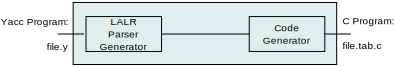
\includegraphics[width=.8\linewidth]{parser_tool}
	\end{center}
\end{frame}

\subsection{Yacc/Bison}

\tableofcontentslide[sectionstyle={show/shaded},subsectionstyle={show/shaded/hide},subsubsectionstyle={show/show/hide/hide}]

\subsubsection{Using Yacc/Bison}

\figureslide{Process of Yacc}{yacc_process}

\begin{frame}[t,fragile]{Structure of a Yacc Program}
	\begin{itemize}
	\item A Yacc program has the following form:
		\begin{lstlisting}[language=C]
		Declarations
		%%
		Translation rules
		%%
		Auxiliary functions
		\end{lstlisting}
	\end{itemize}
	\begin{small}
	\only<1>{\begin{block}{Declarations}
		\begin{itemize}
		\item C ordinary declarations, between \code{\%\{} and \code{\%\}}.
		\item Declarations of tokens with the command \code{\%token}.
		\end{itemize}
	\end{block}}
	\only<2>{\begin{block}{Translation rules}
		Each rule consists of a grammar production and the associated action (note the final semicolon).
		\begin{tabular}{@{}lcl@{}}
		{\textless}head{\textgreater}&:&{\textless}body$_1${\textgreater} \{ {\textless}action$_1${\textgreater} \} \\
		&$|$&{\textless}body$_2${\textgreater} \{ {\textless}action$_2${\textgreater} \} \\
		&&\dots \\
		&$|$&{\textless}body$_n${\textgreater} \{ {\textless}action$_n${\textgreater} \} \\
		&;&
		\end{tabular}
	\end{block}}
	\only<3>{\begin{block}{Auxiliary functions}
		\begin{itemize}
		\item Auxiliary functions are the section where additional C routines should be put.
		\item Note that you must provide the function \code{yylex()}, which is invoking the lexical analyzer (explained later).
		\end{itemize}
	\end{block}}
	\end{small}
\end{frame}

\begin{frame}[fragile]{Example of a Yacc Program}
	\begin{lstlisting}[language=C]
	%{
	    #include <ctype.h>
	%}
	%token DIGIT
	%%
	line   :   expr '\n'        { printf("%d\n", $1); }
	         ;
	expr   :   expr '+' term    { $$ = $1 + $3; }
	         | term
	         ;
	term   :   term '*' factor  { $$ = $1 * $3; }
	         | factor
	         ;
	factor :   '(' expr ')'     { $$ = $2; }
	         | DIGIT
	         ;
	%%
	int yylex() {
	   int c;
	   c = getchar();
	   if (isdigit(c)) {
	      yylval = c - '0'; /* convert char to int */
	      return DIGIT;
	   }
	   return c;
	}
	\end{lstlisting}
\end{frame}

\subsubsection{Ambiguous grammar}

\tableofcontentslide[sectionstyle={show/shaded},subsectionstyle={show/shaded/hide},subsubsectionstyle={show/shaded/hide/hide}]

\begin{frame}{Special Yacc Operators}
	\begin{itemize}
	\item Yacc provides a set of declarations that may be used to remove grammar ambiguity.
	\vfill
	\item Associativity and Precedence:
		\begin{description}
		\item[Left associativity] \%left {\textless}op1{\textgreater} {\textless}op2{\textgreater}\dots
		\item[Right associativity] \%right {\textless}op3{\textgreater} {\textless}op4{\textgreater}\dots
		\item[No associativity] \%nonassoc {\textless}op5{\textgreater} {\textless}op6{\textgreater}\dots
		\item The tokens are given precedences in the order in which they appear in  the declaration part, lower first.
		\item Tokens in the same declaration have the same precedence.
		\end{description}
	\end{itemize}
\end{frame}

\subsubsection{Connecting to Lex}

\tableofcontentslide[sectionstyle={show/shaded},subsectionstyle={show/shaded/hide},subsubsectionstyle={show/shaded/hide/hide}]

\begin{frame}{Use Lex in Conjonction with Yacc}
	\begin{itemize}
	\item Lex was designed to produce lexical analyzers that could be used with Yacc.
	\vfill
	\item The Lex library provides a driver program named \code{yylex()}.
	\vfill
	\item To use Lex in Yacc, you must remove any definition of \code{yylex() }in the Yacc specification; and replace this definition by:
		\begin{center}
		\texttt{\#include \str{"lex.yy.c"}}
		\end{center}
	\vfill
	\item All the tokens defined in the Yacc declaractions are directly available in the Lex program.
	\end{itemize}
\end{frame}

\subsubsection{Error recovery}

\tableofcontentslide[sectionstyle={show/shaded},subsectionstyle={show/shaded/hide},subsubsectionstyle={show/shaded/hide/hide}]

\begin{frame}{Error Production}
	\begin{itemize}
	\item In Yacc, error recovery uses a form of error productions.
	\item First, you must decides what ``major'' nonterminals will have error recovery associated to them.
	\item Typical choices are some subset of the nonterminals generating expressions, statements, blocks, and functions.
%	\item You then add to the grammar error productions of the form: \bnftext{A \bnfbody \tok{error} $\alpha$}, where $A$ is a major nonterminal and $\alpha$ is a string of grammar symbols, perhaps the empty string.
%	\item \tok{error} is a reserved word of Yacc.
	\end{itemize}
%	\begin{example}
%	The following production means that the parser skips just beyond the next semicolon on seeing an error.\\
%	\bnftext{stmt \bnfbody \tok{error}}
%	\end{example}
\end{frame}

\begin{frame}[fragile]{Error Recovery Functions}
	\begin{itemize}
	\item \code{yyerror()} reports an error.
	\item \code{yyerrok()} resets the parser to its normal mode of operation.
	\vfill
	\item \small Here, the error production causes the program to suspend normal parsing when a syntax error is found on an input line.
	\item \small On encountering the error, the parser in the program starts popping symbols from its stack until it encounters a statethat as a shift action on the token error. Then the input is read until the new-line character is read. Then the parser reduces error '{\textbackslash}n' to lines, and emits the diagnotic message ``error message.''
	\end{itemize}
	\begin{lstlisting}[language=C]
	line   :   lines expr '\n'  { printf("%g\n", $2); }
	         | lines '\n'
	         | /* empty or epsilon */
	         | error '\n'       { yyerror("error message");
                                      yyerrok(); }
	\end{lstlisting}
\end{frame}

\subsection{JavaCC}

\tableofcontentslide[sectionstyle={show/shaded},subsectionstyle={show/shaded/hide},subsubsectionstyle={show/show/hide/hide}]

\subsubsection{Using to JavaCC}

\figureslide{Process of JavaCC}{javacc_process}

\begin{frame}[t,fragile]{Structure of a JavaCC Program}
	\begin{itemize}
	\item A JavaCC program has the following form:
		\begin{lstlisting}[language=Java]
		JavaCC options
		PARSER_BEGIN(<parserName>)
		Java compilation unit
		PARSER_END(<parserName>)
		Translation rules
		\end{lstlisting}
	\end{itemize}
	\begin{small}
	\only<1>{\begin{block}{Parser Definition}
		\begin{itemize}
		\item The name that follows ``PARSER\_BEGIN'' and ``PARSER\_END'' must be the same and this identifies the name of the generated parser.
		\end{itemize}
	\end{block}}
	\only<2>{\begin{block}{Options}
		\begin{itemize}
		\item JavaCC options permits to control the behavior of the parser.
		\end{itemize}
	\end{block}}
	\only<3>{\begin{block}{Translation rules}
		The Java compilation unit is a Java code that must contain at least the declaration of the class of the parser: \\
		\dots \\
		\code{\tok{public} \tok{class} {\textless}parser\_name{\textgreater} \{} \\
		\dots \\
		\code{\}} \\
		\dots
	\end{block}}
	\only<4>{\begin{block}{Predefined functions}
		Two functions are automatically generated inside the parser class:
		\begin{itemize}
		\item \code{Token getNextToken()}: returns the next available token.
		\item \code{Token getToken(\tok{int} index)}: returns the ith token ahead.
		\end{itemize}
	\end{block}}
	\only<5>{\begin{block}{Translation rules}
		\begin{itemize}
		\item Java code production (see error recovery for an example),
		\item Regular expression production,
		\item BNF production, or
		\item Token manager declarations (not treated in this lecture).
		\end{itemize}
	\end{block}}
	\end{small}
\end{frame}

\begin{frame}{Define the Regular Expression Productions}
	\begin{definition}
		\code{[{\textless}state\_list{\textgreater}] {\textless}kind{\textgreater} [\tok{IGNORE\_CASE}] \tok{:}} \\
		\code{\{ {\textless}regexpr{\textgreater} $|$ {\textless}regexpr{\textgreater} $|$ \dots \}}
	\end{definition}
	\begin{itemize}
	\item \code{{\textless}state\_list{\textgreater}} specifies the lexer states in which the rule is enabled (default is \code{DEFAULT}).
	\item \tok{IGNORE\_CASE} specifies, by its presence, that if the regular expression is case sensitive or case insensitive.
	\item The regular definitions are defined and used as follows, respectively (The \code{"\#"} before the id indicates that this definition exists solely for the purpose of defining other tokens): \\
		\tok{\textless} [\tok{\#}]id \tok{:} regexpr \tok{\textgreater} \\
		\tok{\textless}id\tok{\textgreater}
	\end{itemize}
\end{frame}

\begin{frame}{Types of Regular Expression Productions \code{{\textless}kind{\textgreater}}}
	\begin{enumerate}
	\item[TOKEN] describes tokens in the grammar. The token manager creates a Token object for each match of such a regular expression and returns it to the parser.
	\vfill
	\item[SPECIAL\_TOKEN] like tokens, except that they do not have significance during parsing, ie. the BNF productions ignore them.
	\vfill
	\item[SKIP] simply skipped (ignored) by the token manager.
	\vfill
	\item[MORE] Sometimes it is useful to gradually build up a token to be passed on to the parser. Matches to this kind of regular expression are stored in a buffer until the next \tok{TOKEN} or \tok{SPECIAL\_TOKEN} match.
	\end{enumerate}
\end{frame}

\begin{frame}{Attributes of the Predefined \code{Token} Class}
	\begin{itemize}
	\item \code{\tok{int} kind} \\
		This is the index for this kind of token in the internal representation scheme of JavaCC. It may be replaced by a constant.
	\vfill
	\item \code{\tok{int} beginLine, beginColumn, endLine, endColumn} \\
		The beginning and ending positions of the token as it appeared in the input stream.
	\vfill
	\item \code{\tok{String} image} \\
		The image of the token as it appeared in the input stream.
	\vfill
	\item \code{\tok{Token} next} \\
		A reference to the next regular (non-special) token from the input stream.
	\end{itemize}
\end{frame}

\begin{frame}{Methods of the Predefined \code{Token} Class}
	\begin{itemize}
	\item \code{\tok{Object} getValue()} \\
		An optional attribute value of the \code{Token}. Tokens which are not used as syntactic sugar will often contain meaningful values that will be used later on by the compiler or interpreter. This attribute value is often different from the image. Any subclass of Token that actually wants to return a non-null value can override this method as appropriate.
	\vfill
	\item \code{\tok{static} \tok{final} Token newToken(\tok{int} ofKind)} \\
		\code{\tok{static} \tok{final} Token newToken(\tok{int} ofKind, \tok{String} image)} \\
		Returns a new token object as its default behavior.
	\end{itemize}
\end{frame}

\begin{frame}[t]{BNF Productions}
	\begin{definition}\small
		\code{{\textless}access\_modifier{\textgreater} {\textless}return\_type{\textgreater}} \\
		\code{{\textless}identifier{\textgreater} \tok( {\textless}parameters{\textgreater} \tok) \tok:} \\
		\code{{\textless}java\_block{\textgreater}} \\
		\code{\tok\{ {\textless}expansion\_choices{\textgreater} \tok\}}
	\end{definition}
	\begin{itemize}
	\item The name of the non-terminal is the name of the method, and the parameters and return value declared are the means to pass values up and down the parse tree.
	\item Non-terminals on the right hand sides of productions are written as method calls, so the passing of values up and down the tree are done using exactly the same paradigm as method call and return.
	\item The default access modifier for BNF productions is public.
	\end{itemize}
\end{frame}

\begin{frame}[t]{Heads of the Productions}
	\begin{definition}\small
		\code{{\textless}access\_modifier{\textgreater} {\textless}return\_type{\textgreater}} \\
		\code{{\textless}identifier{\textgreater} \tok( {\textless}parameters{\textgreater} \tok) \tok:} \\
		\code{{\textless}java\_block{\textgreater}} \\
		\code{\tok\{ {\textless}expansion\_choices{\textgreater} \tok\}}
	\end{definition}
	\begin{itemize}
	\item The name of the non-terminal is the name of the method, and the parameters and return value declared are the means to pass values up and down the parse tree.
	\item Non-terminals on the right hand sides of productions are written as method calls, so the passing of values up and down the tree are done using exactly the same paradigm as method call and return.
	\item The default access modifier for BNF productions is public.
	\end{itemize}
\end{frame}

\begin{frame}[t]{Bodies of the Productions}
	\begin{definition}\small
		\code{{\textless}access\_modifier{\textgreater} {\textless}return\_type{\textgreater}} \\
		\code{{\textless}identifier{\textgreater} \tok( {\textless}parameters{\textgreater} \tok) \tok:} \\
		\code{{\textless}java\_block{\textgreater}} \\
		\code{\tok\{ {\textless}expansion\_choices{\textgreater} \tok\}}
	\end{definition}
	\begin{description}
	\item[Java block] arbitrary Java declarations and code put at the beginning of the method generated for the Java non-terminal.
	\item[Expansion choices] a sequence of expansion units. Each nonterminal is written as a function call. Semantic actions are Java blocks inside this part of the BNF production.
	\end{description}
\end{frame}

\begin{frame}[fragile]{Example of JavaCC File \insertcontinuationwith{1}}
	\begin{lstlisting}{language=Java}
	PARSER_BEGIN(CalculatorParser)
	    public class CalculatorParser {
	    }
	PARSER_END(CalculatorParser)

	SKIP: {
	       " "
	    |  "\t"
	    |  "\n"
	    |  "\r"
	}

	TOKEN :
	{
	     <DIGIT : [0-9]>
	}
	\end{lstlisting}
\end{frame}

\begin{frame}[fragile]{Example of JavaCC File \insertcontinuationwith{2}}
	\begin{lstlisting}{language=Java}
	private void line() :
	{
	    int e;
	}
	{ e = expr()       { System.out.println(e); }
	}

	private int expr() :
	{
	    int e, t;
	}
	{ e = expr() "+" t = term()   { return e+t; }
	  | t = term()                { return v; }
	}
	\end{lstlisting}
\end{frame}

\begin{frame}[fragile]{Example of JavaCC File \insertcontinuationwith{3}}
	\begin{lstlisting}{language=Java}
	private int term() :
	{
	    int t, f;
	}
	{ t = term() "*" f = factor()   { return t*f; }
	  | f = factor()                { return f; }
	}

	private int factor() :
	{
	    int e, d;
	}
	{ "(" e = expr() ")"            { return e; }
	  | d = <DIGIT>                 { return Integer.parseInt(d.image); }
	}
	\end{lstlisting}
\end{frame}

\subsubsection{Error recovery}

\tableofcontentslide[sectionstyle={show/shaded},subsectionstyle={show/shaded/hide},subsubsectionstyle={show/shaded/hide/hide}]

\begin{frame}{Error Reporting with JavaCC}
	\begin{itemize}
	\item Simply modify the file \texttt{ParseException.java} to do what you want it to do. Typically, you would modify the \code{getMessage} method to do your own customized error reporting.
	\item All information regarding these methods can be obtained from the comments in the generated files \texttt{ParseException.java} and \texttt{TokenMgrError.java}.
	\vfill
	\item There is a method in the generated parser called \code{generateParseException()}.
	\item You can call this method anytime you wish to generate an object of type \code{ParseException}. This object will contain all the choices that the parser has attempted since the last successfully consumed token.
	\end{itemize}
\end{frame}

\begin{frame}{Error Recovery with JavaCC}
	JavaCC offers two kinds of error recovery:
	\vfill
	\begin{enumerate}
	\item[Shallow recovery] recovers if none of the current choices have succeeded in being selected.
	\vfill
	\item[Deep recovery] is when a choice is selected, but then an error happens sometime during the parsing of this choice.
	\end{enumerate}
\end{frame}

\begin{frame}[fragile]{Shallow Error Recovery}
	When no token found, we want to skip until the next given symbol (semi-column). \\
	\begin{lstlisting}{language=Java}
	TOKEN : { <SEMICOLON: ";"> }
	private void stm() :
	{}
	{ ifStm()
	  | whileStm()
	}
	\end{lstlisting}
	\begin{center}
\includegraphics[height=2em]{bottomarrow}\end{center}
	\begin{lstlisting}{language=Java}
	TOKEN : { <SEMICOLON: ";"> }
	private void stm() :
	{}
	{ ifStm()
	  | whileStm()
	  | whileStm()
	  | error_skipto(SEMICOLON)
	}
	\end{lstlisting}
\end{frame}

\begin{frame}[fragile]{Definition of the function \code{error\_skipto()}}
	\begin{itemize}
	\item \code{error\_skipto()} is a nonterminal that must be define prior to its first usage.
	\item To do so, we must use the following JAVACODE rule.
	\end{itemize}
	\begin{lstlisting}{language=Java}
	JAVACODE
	void error_skipto(int kind) {
	    ParseException e = generateParseException()
	    System.err.println(e);
	    Token t;
	    do {
	        t = getNextToken();
	    }
	    while (t.kind != kind);
	}
	\end{lstlisting}
\end{frame}

\begin{frame}[fragile]{Deep Error Recovery}
	When error occured (even deeper in the parse tree), we want to recover. \\
	\begin{lstlisting}{language=Java}
	TOKEN : { <SEMICOLON: ";"> }
	private void stm() :
	{}
	{ ifStm()
	  | whileStm()
	}
	\end{lstlisting}
	\mbox{}\hfill
\includegraphics[height=2em]{bottomarrow}\hfill\mbox{}
	\begin{lstlisting}{language=Java}
	TOKEN : { <SEMICOLON: ";"> }
	private void stm() :
	{}
	{ try {
	      ifStm()
	      | whileStm()
	      | whileStm()
	  } catch(ParseException e) {
	      error_skipto(e, SEMICOLON);
	  }
	}
	\end{lstlisting}
\end{frame}

\begin{frame}[fragile]{Definition of the function \code{error\_skipto()}}
	\begin{lstlisting}{language=Java}
	JAVACODE
	void error_skipto(ParseException e, int kind) {
	    System.out.println(e);
	    Token t;
	    do {
	        t = getNextToken();
	    }
	    while (t.kind != kind);
	}
	\end{lstlisting}
\end{frame}

\section{Conclusion}

\tableofcontentslide[sectionstyle={show/shaded},subsectionstyle={hide/hide/hide},subsubsectionstyle={hide/hide/hide/hide}]

\begin{frame}[t,allowframebreaks]{Key Concepts in the Chapter}
	\begin{small}
	\begin{description}
	\item[Parsers] A parser takes as input tokens from the lexical analyzer and treats the token names as terminal symbols of a context-free grammar. The parser then constructs a parse tree for its input sequence of tokens; the parse tree may be constructed figuratively or literally.
	\item[Context-Free Grammars] A grammar specifies a set of terminal symbols (inputs), another set of nonterminals (symbols representing syntactic constructs), and a set of productions, each of which gives a way in which strings represented by one nonterminal can be constructed from terminal symbols and strings represented by certain other nonterminals. A production consists of a head (the nonterminal to be replaced) and a body (the replacing string of grammar symbols).
	\item[Derivations] The process of starting with the start-nonterminal of a grammar and successively replacing it by the body of one its productions is called derivation. If the leftmost (or rightmost) nonterminal is always replaced, then the derivation is called leftmost (resp. rightmost.)
	\item[Parse Trees] A parse tree is a picture of a derivation, in which there is a node for each nonterminal that appears in the derivation. The children of a node are the symbols by which that nonterminal is replaced in the derivation. There is a one-to-one correspondence between parse trees, leftmost derivation, and rightmost derivations of the same terminal string.
	\item[Ambiguity] A grammar for which some terminal string has two or more different parse tree is said to be ambiguous.
	\item[Top-Down and Bottom-Up Parsing] Parsers are generally distinguished by whether they work top-down or bottom-up. Top-down parsers include recursive-descent and LL parsers, while the most common forms of bottom-up parsers are LR parsers.
	\item[Design of Grammars] Grammars suitable for top-down parsing often are harder to design than those used by bottom-up parsers. It is necessary to eliminate left-recursion. We also must left-factor/group productions for the same nonterminal that have a common prefix in the body.
	\item[Recursive-Descent Parsers] These parsers use a procedure for each nonterminal.
	\item[$LL(1)$ Parsers] A grammar such that it is possible to choose the correct production with which to expand a given nonterminal, looking only at the next input symbol, is called $LL(1)$. These grammars allow us to construct a predictive parsing table that gives, for each nonterminal and each lookahead symbol, the correct choice of production.
	\item[Shift-Reduce Parsing] Bottom-up parsers generally operate by choosing on the basis of the next input symbol and the contents of the stack, whether to shift the next input onto the stack, or to reduce some symbols at the top of the stack. A reduce takes a production body at the top of the stack and replaces it by the head of the production.
	\item[Viable Prefixes] In shift-reduce parsing, the stack contents are always a viable prefix, ie. a prefix of some right-sentential form that ends no further right than the end of the handle of that right-sentential form. The handler is the substring that was introduced in the last step of the rightmost derivation of that sentential form.
	\item[Valid Items] An item is a production with a dot somewhere in the body. An item is valid for a viable prefix if the production of that item is used to generate the handler, and the viable prefix includes all those symbols to the left of the dot.
	\item[$LR$ Parsers] Each of the several kinds of LR parsers operate by first constructing the sets of valid items (called LR states) for all possible viable prefixes, and keeping track of the state for each prefix on the stack. The set of valid items guide the shift-reduce parsing decision.
	\item[Simple $LR$ Parsers] In an $SLR$ parser, we perform a reduction implied by a valid item with a dot at the right end, provided the lookahead symbol can follow the head of that production in some sentential form.
	\item[Canonical-$LR$ Parsers] This more complex form of $LR$ parser uses items that are augmented by the set of lookahead symbols that can follow the use of the underlying production. A canonical-$LR$ parser can avoid some of the parsing-action conflicts that are present in $SLR$ parsers, but often has many more states than the $SLR$ parser for the same grammar.
	\end{description}
	\end{small}
\end{frame}

\begin{frame}[t,allowframebreaks]{\bibname\ of the Chapter}%
	\tiny%
	\putbib[bibliographies/chapter3]%
\end{frame}%

\end{bibunit}
